\documentclass[letterpaper,12pt,notitlepage,twoside]{report}

\newcommand{\watermark}{MLOps}
\newcommand{\booktopic}{Machine Learning Operations}
\newcommand{\lastname}{Okoli}
\usepackage{NoteStyle}
\usepackage{placeins}
\usepackage{listings}
\usepackage{pifont}

\definecolor{firebrick}{rgb}{0.7, 0.13, 0.13}

\definecolor{codegreen}{rgb}{0,0.6,0}
\definecolor{codegray}{rgb}{0.5,0.5,0.5}
\definecolor{codepurple}{rgb}{0.58,0,0.82}
\definecolor{backcolour}{rgb}{0.95,0.95,0.92}

\lstdefinestyle{mystyle}{
    backgroundcolor=\color{backcolour},   
    commentstyle=\color{codegreen},
    keywordstyle=\color{magenta},
    numberstyle=\tiny\color{codegray},
    stringstyle=\color{codepurple},
    basicstyle=\ttfamily\footnotesize,
    breakatwhitespace=false,         
    breaklines=true,                 
    captionpos=b,                    
    keepspaces=true,                 
    numbers=left,                    
    numbersep=5pt,                  
    showspaces=false,                
    showstringspaces=false,
    showtabs=false,                  
    tabsize=2
}

% Prevents hypenation 
\tolerance=1
\emergencystretch=\maxdimen
\hbadness=10000


\lstset{style=mystyle}

\title{Machine Learning Operations}
\author{Chuks Okoli}
\date{\footnotesize Last Updated: \today}

\hypersetup{
  pdftitle={Machine Learning Operations},
  pdfauthor={Chuks Okoli},
  pdfsubject={},
}

% ToC on the title page:
% https://tex.stackexchange.com/a/45863
\makeatletter
\newcommand*{\toccontents}{\@starttoc{toc}}
\makeatother

\begin{document}

\begin{titlepage}
  \pagestyle{plain}
  \maketitle
  \setcounter{tocdepth}{2}

  \pdfbookmark[section]{\contentsname}{toc}
  \toccontents
  % Separate page:
  % \tableofcontents
\end{titlepage}

%------------------- Chapter 1: Introduction  -----------------%
\chapter{Introduction} \label{ch:1}

\firstletter{Hello there}, and welcome to \booktopic. This work is a culmination of hours of effort to create my reference for machine learning operations. All of the explanations are in my own words but majority of the content are based on Alexey Grigorev's DataTalksClub \href{https://github.com/DataTalksClub/mlops-zoomcamp}{MLOps Zoomcamp course}.

\begin{mathaside}[frametitle=\mathtitle{Explaining MLOps to a \color{firebrick}{5 year old}}]
\textit{Imagine you have a magical garden. In this garden, you have a special plant that can grow different kinds of fruits, but you need to take good care of it.}

\textit{MLOps is like having a magical gardener to help you. This gardener does three important things:}
\begin{enumerate}
    \item \textit{\textbf{Teaching the Plant}: The gardener shows the plant pictures of different fruits (like apples, oranges, and bananas) so it can learn to grow them. This is like the gardener helping the plant understand what to do. In MLOps, this is called training a machine learning model.}
    
    \item \textit{\textbf{Taking Care of the Garden}: The gardener makes sure the soil is rich, the water is just right, and there are no weeds. The gardener also provides the plant with the best tools and instructions to grow healthy fruits. In MLOps, this is called managing the infrastructure for the machine learning model.}
    
    \item \textit{\textbf{Sharing the Fruits}: Once the plant grows the fruits, the gardener picks them and puts them in baskets for everyone to enjoy. The gardener makes sure the fruits are easy to find and delicious. In MLOps, this is called deploying the model so it can be used for something useful.}
\end{enumerate}

\textit{Here's the magical part: The gardener watches over the garden to make sure everything is running smoothly. If a bug tries to eat the plant or if the plant stops growing fruits, the gardener fixes the problem right away.}

\textit{So, MLOps is like having a magical gardener who helps your special plant (machine learning model) stay happy, healthy, and productive, making sure it grows the best fruits for everyone to enjoy!}
\end{mathaside}


\section{What is MLOps?}
\inspiration{MLOps, also known as DevOps for machine learning, is an umbrella term that encompasses philosophies, practices, and technologies that are related to implementing machine learning lifecycles in a production environment.}{Microsoft Blog}{}

Machine Learning Operations (MLOps) is a set of best practices for putting machine learning models into production. The process for a machine learning project involves:
\begin{itemize}
	\item Design - define if machine learning is the right tool for solving the problem
	\item Train - train the model to find the best possible model
	\item Operate - deploy the model,  and monitor degradation or quality of the model
\end{itemize}
MLOps is a set of practices for automating everything and working together as a team on a machine learning project.

 \begin{funfact}[frametitle=\facttitlep{Fun Fact}{MLOps Principles}]
As machine learning and AI become more common in software, it's important to create guidelines and tools for testing, deploying, managing, and monitoring ML models in real-world use. This is where MLOps comes in. It helps prevent ``technical debt'' in machine learning projects by ensuring smooth operation and maintenance of models throughout their lifecycle.
\end{funfact}

MLOps helps to manage and orchestrate the end-to-end machine learning lifecycle by ensuring models are consistently accessible, reproducible, and scalable. It focuses on automating deployment and monitoring of ML pipelines while optimizing the model development process.

The three-phase approach to implementing machine learning (ML) solutions are:
\begin{itemize}
\item \textbf{Business Understanding and Design}: This phase involves identifying user needs, designing ML solutions to address them, and assessing project development. Prioritizing ML use cases and defining data requirements are key steps. The architecture of the ML application, serving strategy, and testing suite are designed based on functional and non-functional requirements.
\item \textbf{ML Experimentation and Development}: This phase focuses on verifying the applicability of ML by implementing Proof-of-Concept models. It involves iteratively refining ML algorithms, data engineering, and model engineering to deliver a stable, high-quality ML model for production.
\item \textbf{ML Operations}: Here, the emphasis is on deploying the developed ML model into production using established DevOps practices. Testing, versioning, continuous delivery, and monitoring are essential aspects of this phase.
\end{itemize}
These phases are interconnected, with design decisions influencing experimentation and deployment options.

\begin{figure}[h]
	\centering
	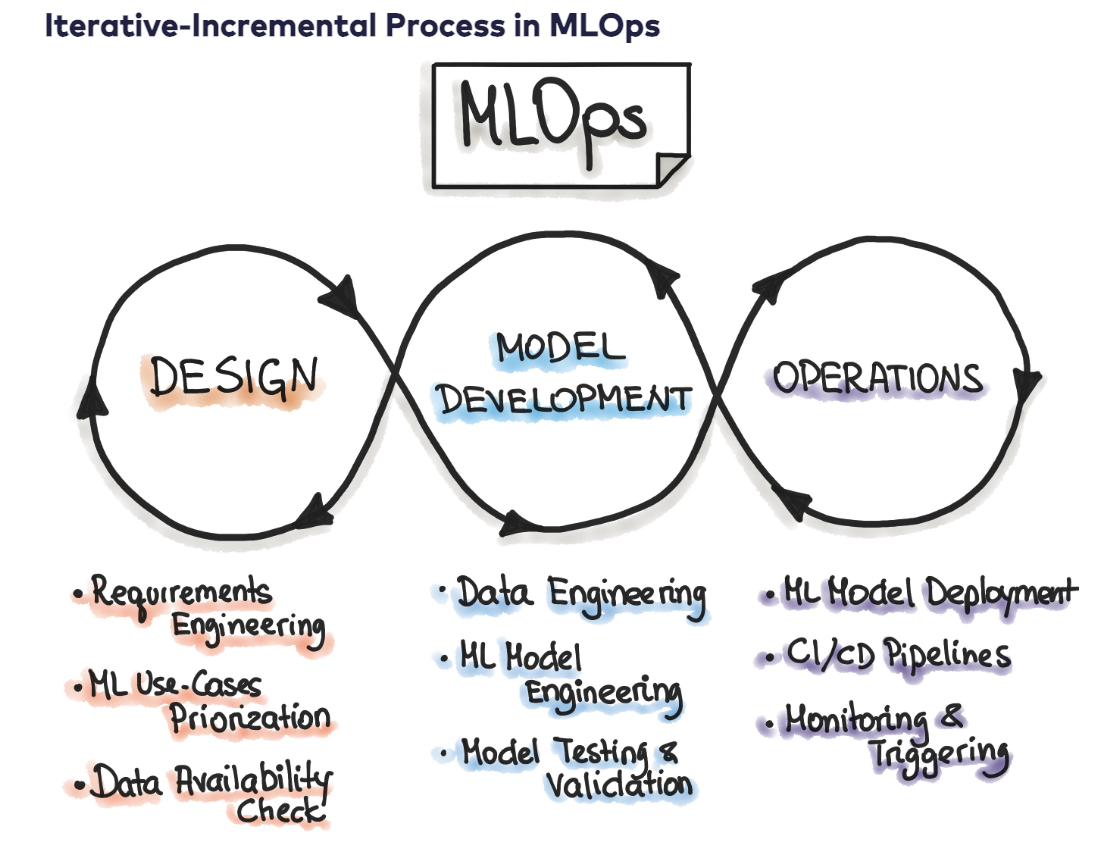
\includegraphics[width=\textwidth]{Images/Iterative MLOps.png}
	\caption{The complete MLOps process includes three broad phases of ``Designing the ML-powered application'', ``ML Experimentation and Development'',  and ``ML Operations''.}
	\label{fig:1}
\end{figure}
\FloatBarrier

MLOps leverages various tools to simplify the machine learning lifecycle.
\begin{itemize}[label={--}]
\item \textbf{Machine learning frameworks} like Kubernetes, TensorFlow and PyTorch for model development and training.
\item \textbf{Version control systems} like Git for code and model version tracking.
\item \textbf{CI/CD tools} such as Jenkins or GitLab CI/CD for automating model building, testing and deployment.
\item \textbf{MLOps platforms} like Kubeflow and MLflow manages model lifecycles, deployment and monitoring.
\item \textbf{Cloud computing platforms} like AWS, Azure and IBM Cloud provide scalable infrastructure for running and managing ML workloads.
\end{itemize}


\section{Environment Preparation}
\subsection{Configuring Environment with GitHub Codespaces}
To configure the environment using GitHub codespaces, first create a repository on GitHub, give the repository a name, add a ``README'' file and a \texttt{.gitignore} template, choose a license and create the repo. In the repo main page, click on \texttt{Create codespace on main} as shown in \textbf{Fig. \ref{fig:2}}.
\begin{figure}[h]
	\centering
	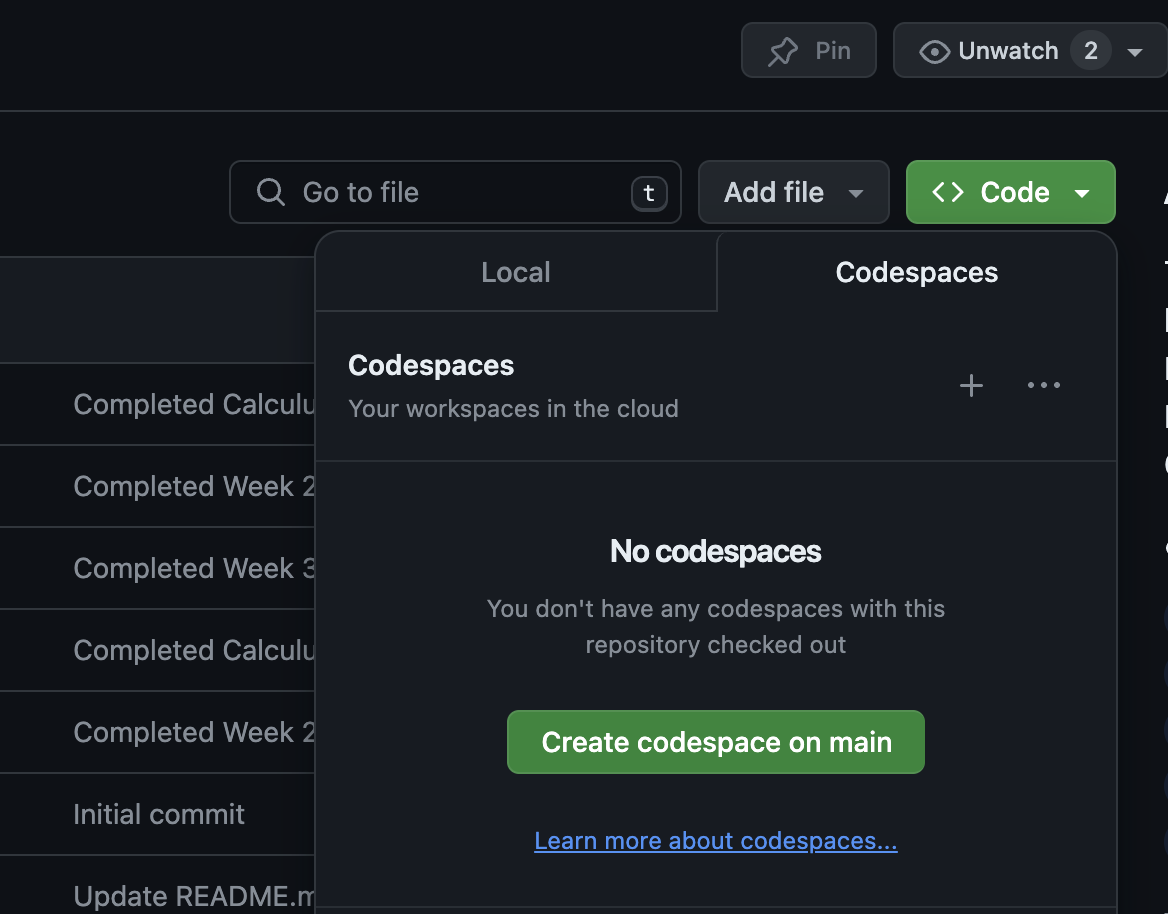
\includegraphics[width=0.5\textwidth]{Images/Codespaces.png}
	\caption{GitHub Codespaces setup}
	\label{fig:2}
\end{figure}
\FloatBarrier

A connection to Visual Studio Code can be made through Codespaces.  Start a new terminal, change directory to the workspaces and download and install Anaconda distribution of python in it using the step below.
 \begin{itemize}
\item \textbf{Step 1}: Download and install the Anaconda distribution of Python 
\begin{lstlisting}[language=python, numbers=none]
wget https://repo.anaconda.com/archive/Anaconda3-2022.05-Linux-x86_64.sh
\end{lstlisting}
\item \textbf{Step 2}: Run this command: 
\begin{lstlisting}[language=python, numbers=none]
bash Anaconda3-2022.05-Linux-x86_64.sh
\end{lstlisting}

After installing Anaconda, initialize it. In a new terminal, confirm that Anaconda is running in the workspaces
\begin{lstlisting}[language=python, numbers=none]
(base) @your_username -> /workspaces/mlops-zoomcamp-2024 (main) $ which python
/home/codespace/anaconda3/bin/python
\end{lstlisting}
\item \textbf{Step 3}: Make sure to install \texttt{pyarrow} in order to download parquet file
\begin{lstlisting}[language=python, numbers=none]
!pip install pyarrow
\end{lstlisting}
\item \textbf{Step 4}: Run jupyter notebook
\begin{lstlisting}[language=python, numbers=none]
jupyter notebook
\end{lstlisting}
\end{itemize}

\subsection{Configuring Environment with Amazon Web Service (AWS)}
To install using AWS,  create an account in AWS, go to EC2 and create an instance. Select the OS to use e.g. Ubuntu with 64-bit(x86) architecture. Select the instance type that will be sufficient for your project. Configure the cloud resources and launch. \\
Recommended development environment: Linux

 \begin{itemize}
\item \textbf{Step 1}: Download and install the Anaconda distribution of Python 
\begin{lstlisting}[language=python, numbers=none]
wget https://repo.anaconda.com/archive/Anaconda3-2022.05-Linux-x86_64.sh
bash Anaconda3-2022.05-Linux-x86_64.sh
\end{lstlisting}
\item \textbf{Step 2}: Update existing packages
\begin{lstlisting}[language=python, numbers=none]
sudo apt update
\end{lstlisting}
\item \textbf{Step 3}: Install Docker
\begin{lstlisting}[language=python, numbers=none]
sudo apt install docker.io
\end{lstlisting}
To run docker without sudo:
\begin{lstlisting}[language=python, numbers=none]
sudo groupadd docker
sudo usermod -aG docker \$USER
\end{lstlisting}
\item \textbf{Step 4}: Install Docker Compose \\
Install docker-compose in a separate directory
\begin{lstlisting}[language=python, numbers=none]
mkdir soft
cd soft
\end{lstlisting}
To get the latest release of Docker Compose, go to https://github.com/docker/compose and download the release for your OS.
\begin{lstlisting}[language=python, numbers=none]
wget https://github.com/docker/compose/releases/download/v2.5.0/docker-compose-linux-x86_64 -O docker-compose
\end{lstlisting}
Make it executable
\begin{lstlisting}[language=python, numbers=none]
chmod +x docker-compose
\end{lstlisting}
Add the soft directory to PATH. Open the .bashrc file with nano:
\begin{lstlisting}[language=python, numbers=none]
nano ~/.bashrc
\end{lstlisting}
In .bashrc, add the following line:
\begin{lstlisting}[language=python, numbers=none]
export PATH="${HOME}/soft:${PATH}"
\end{lstlisting}
Save it and run the following to make sure the changes are applied:
\begin{lstlisting}[language=python, numbers=none]
source ~/.bashrc
\end{lstlisting}
\item \textbf{Step 5}: Run Docker
\begin{lstlisting}[language=python, numbers=none]
docker run hello-world
\end{lstlisting}
\end{itemize}

\section{Model Development}
\subsection{Taxi trip prediction with machine learning}
    \begin{example}[frametitle=\extitle{TLC Trip Prediction}]
      In this section, we use machine learning to predict the trip duration for trips in New York. The data used were collected from the \href{https://www.nyc.gov/site/tlc/about/tlc-trip-record-data.page}{NYC Taxi and Limousine Commission (TLC)}. This dataset contains yellow and green taxi trip records include fields capturing pick-up and drop-off dates/times, pick-up and drop-off locations, trip distances, itemized fares, rate types, payment types, and driver-reported passenger counts. The data is stored in the PARQUET format.  We built a simple linear regression model and save the model as a pickle file for subsequent use later one.  See the \href{https://github.com/chuksoo/mlops-zoomcamp-2024/blob/main/01%20-%20Intro/duration-prediction.ipynb}{duration prediction notebook}.
    \end{example}

We can download parquet file using:
\begin{lstlisting}[language=python, numbers=none]
# download parquet data
!wget https://d37ci6vzurychx.cloudfront.net/trip-data/green_tripdata_2021-01.parquet
\end{lstlisting}

\section{MLOps Maturity Model}
The MLOps maturity model helps clarify the Development Operations (DevOps) principles and practices necessary to run a successful MLOps environment.  The maturity is the extent to which MLOps is implemented in a team. The MLOps maturity model encompasses five levels of technical capability.

% Please add the following required packages to your document preamble:
\begin{table}[H]
\resizebox{\columnwidth}{!}{%
\begin{tabular}{cp{2.5cm}p{7.0cm}p{7.0cm}}
\hline
Level & Description                     & Highlights                                                                                                                                                                                                                                         & Technology                                                                                                                                                                                   \\ \hline \hline
0     & No MLOps & \begin{itemize}[noitemsep, topsep=0pt]
    \item Hard to manage lifecycle
    \item Disparate teams
    \item Systems as ``black boxes''
\end{itemize}                 & \begin{itemize}[noitemsep, topsep=0pt]
    \item Manual builds/deployments
    \item Manual testing
    \item No centralized tracking
\end{itemize} \\ \hline
1     & DevOps but no MLOps            & \begin{itemize}[noitemsep, topsep=0pt]
   \item Less painful releases
    \item Limited feedback
    \item Hard to reproduce results
\end{itemize}              & \begin{itemize}[noitemsep, topsep=0pt]
    \item Automated builds
    \item Automated tests for application code
\end{itemize} \\ \hline
2     & Automated Training              & \begin{itemize}[noitemsep, topsep=0pt]
   \item Managed, traceable training
    \item Easy to reproduce model
    \item Low friction releases
\end{itemize}                      & \begin{itemize}[noitemsep, topsep=0pt]
    \item Automated model training
    \item Centralized tracking of model training performance
    \item Model management
\end{itemize} \\ \hline
3     & Automated Deployment     & \begin{itemize}[noitemsep, topsep=0pt]
    \item Releases are low friction and automatic
    \item Full traceability from deployment back to original data
    \item Entire environment managed: train > test > production
\end{itemize}                            & \begin{itemize}[noitemsep, topsep=0pt]
   \item Integrated A/B testing
    \item Automated tests for all code
    \item Centralized tracking
\end{itemize} \\ \hline
4     & Full MLOps Automated Operations & \begin{itemize}[noitemsep, topsep=0pt]
    \item Fully automated, monitored
    \item Systems provide improvement information
    \item Zero-downtime
\end{itemize} & \begin{itemize}[noitemsep, topsep=0pt]
    \item Automated training/testing
    \item Centralized metrics
\end{itemize}                                                              \\ \hline \hline
\end{tabular}%
}
\caption{Machine Learning operations maturity model (culled from \href{https://learn.microsoft.com/en-us/azure/architecture/ai-ml/guide/mlops-maturity-model}{Microsoft Blog}}
\label{tab:my-table}
\end{table}

%--------------- Chapter 2: Experiment Tracking and Model Management -----------%
\chapter{Experiment Tracking and Model Management} \label{ch:2}

\inspiration{MLOps is critical for the success of AI projects because it allows teams to iterate quickly and deploy machine learning models reliably and at scale.}{Andrew Ng}{}

\section{Introduction to Experiment Tracking}

 \begin{funfact}[frametitle=\facttitlep{Fun Fact}{MLflow}]
MLflow is an open-source platform that helps manage the end-to-end machine learning lifecycle. It provides a set of tools to streamline and automate various stages of the machine learning process, from experimentation to deployment. 
\end{funfact}

Machine Learning experiment is the process of building an ML model. Experiment run represents each trial in an ML experiment. A run artifact is any file associated with an ML run. The experiment metadata is all the information related to the experiment. \emph{Experiment tracking} is the process of keeping track of all the \textbf{relevant information} from an \textbf{ML experiment}, which includes:
\begin{itemize}[noitemsep, topsep=0pt]
	\item Source code
	\item Environment
	\item Data
	\item Models
	\item Hyperparameters
	\item Metrics
\end{itemize}

    \begin{mathaside}[frametitle=\mathtitle{Why is Experiment Tracking \color{firebrick}{so important}}]
      Experiment tracking is important because of \textbf{Reproducibility}, \textbf{Organization}, and \textbf{Optimization}
    \end{mathaside}

Experiment tracking is done using MLflow. MLflow is ``an open source platform for the machine learning lifecycle''. In practice, it's just a Python package that can be installed with pip, and it contains four main modules:
\begin{itemize}[noitemsep, topsep=0pt]
	\item Tracking
	\item Models
	\item Model Registry
	\item Projects
\end{itemize}

The MLflow Tracking module allows you to organize your experiments into runs, and to keep track of:
\begin{itemize}[noitemsep, topsep=0pt]
	\item Parameters
	\item Metrics
	\item Metadata
	\item Artifacts
	\item Models
\end{itemize}

Along with this information, MLflow automatically logs extra information about the run:
\begin{itemize}[noitemsep, topsep=0pt]
	\item Source code i.e., the name of the file that was used to run the experiment
	\item Version of the code (git commit)
	\item Start and end time
	\item Author
\end{itemize}

\subsection{How MLflow Helps Manage Machine Learning Experiments}
Here are some key ways in which MLflow can help with machine learning experiments:
\subsubsection{Experiment Tracking}
MLflow Tracking allows you to log and query experiments using APIs or a web-based interface. Key features include:

\begin{itemize}
    \item \textbf{Log Parameters and Metrics:} Easily log hyperparameters, metrics, and artifacts (such as model files) for each run.
    \item \textbf{Organize and Compare Runs:} Organize runs by experiments and compare results visually.
    \item \textbf{Search and Query:} Search and filter experiments using a web UI or API, allowing you to quickly find runs with specific attributes.
\end{itemize}

\subsubsection{Reproducibility}
MLflow promotes reproducibility of experiments by providing:

\begin{itemize}
    \item \textbf{Code Versioning:} Integrates with version control systems (like Git) to log the version of the code that produced a particular run.
    \item \textbf{Environment Management:} Capture and reproduce the software environment using Conda environments or Docker images.
    \item \textbf{Artifacts:} Store and retrieve artifacts such as datasets, models, and images, ensuring all elements of an experiment are preserved.
\end{itemize}

\subsubsection{Model Management}
MLflow Models facilitate model packaging, sharing, and deployment:

\begin{itemize}
    \item \textbf{Standardized Format:} Save models in a standardized format that includes the model itself along with its dependencies and environment.
    \item \textbf{Multi-Platform Support:} Export models to various formats (e.g., TensorFlow, PyTorch, scikit-learn) and deploy them to different environments (e.g., cloud services, Docker).
    \item \textbf{Model Registry:} Register and version models, track model lineage, and transition models through stages (e.g., ``staging'', ``production'').
\end{itemize}

\subsubsection{Deployment}
MLflow provides tools for deploying models to various platforms:

\begin{itemize}
    \item \textbf{Built-in Deployment Options:} Deploy models to cloud platforms like AWS SageMaker, Azure ML, and Google Cloud ML Engine.
    \item \textbf{Custom Deployments:} Create custom deployment logic using the MLflow REST API or the command-line interface (CLI).
    \item \textbf{Batch and Real-Time Serving:} Support for both batch and real-time serving of models, enabling various deployment scenarios.
\end{itemize}

\subsubsection{Collaboration}
MLflow facilitates collaboration among team members by providing:

\begin{itemize}
    \item \textbf{Centralized Tracking Server:} A centralized tracking server where team members can log and view experiment runs.
    \item \textbf{Sharing and Collaboration:} Share results, models, and insights easily within the team, fostering better collaboration and knowledge sharing.
    \item \textbf{Integration with CI/CD:} Integrate MLflow with continuous integration and continuous deployment (CI/CD) pipelines for automated testing and deployment of models.
\end{itemize}

\subsubsection{Scalability}
MLflow is designed to scale with your needs:

\begin{itemize}
    \item \textbf{Distributed Tracking:} Support for tracking experiments across distributed environments, making it suitable for large-scale machine learning projects.
    \item \textbf{Flexible Storage Options:} Use various backend storage systems for logging data, including file systems, databases, and cloud storage.
\end{itemize}

By integrating MLflow into your machine learning workflow, you can enhance the management, reproducibility, and deployment of your experiments. It provides a comprehensive set of tools that streamline the entire lifecycle of machine learning models, making it easier to track, reproduce, and deploy models at scale.


\section{Experiment tracking with MLflow}
To start experiment tracking, we need to create a conda environment for tracking experiment and activate it.
\begin{lstlisting}[language=python, numbers=none]
conda create -n exp-tracking-env python=3.9
conda activate exp-tracking-env
\end{lstlisting}

Once the environment is activated, install the ``requirements.txt'' file using:
\begin{lstlisting}[language=python, numbers=none]
pip install -r requirements.txt
\end{lstlisting}

Check the installed packages using:
\begin{lstlisting}[language=python, numbers=none]
pip list
\end{lstlisting}

To launch mlflow, and store all the artifacts in an sqlite database, we run:
\begin{lstlisting}[language=python, numbers=none]
mlflow ui --backend-store-uri sqlite:///mlflow.db --port 5001
\end{lstlisting}

If you encounter error when launching mlflow, use:
\begin{lstlisting}[language=python, numbers=none]
ps -A | grep gunicorn
\end{lstlisting} to view the processes using the port and kill them with:
\begin{lstlisting}[language=python, numbers=none]
kill <process number>
\end{lstlisting} before re-launching mlflow. 


To access mlflow ui, open \href{http://127.0.0.1:5001} in your browser. The mlflow interface is seen in \textbf{Fig. \ref{fig:3}}.
\begin{figure}[h]
	\centering
	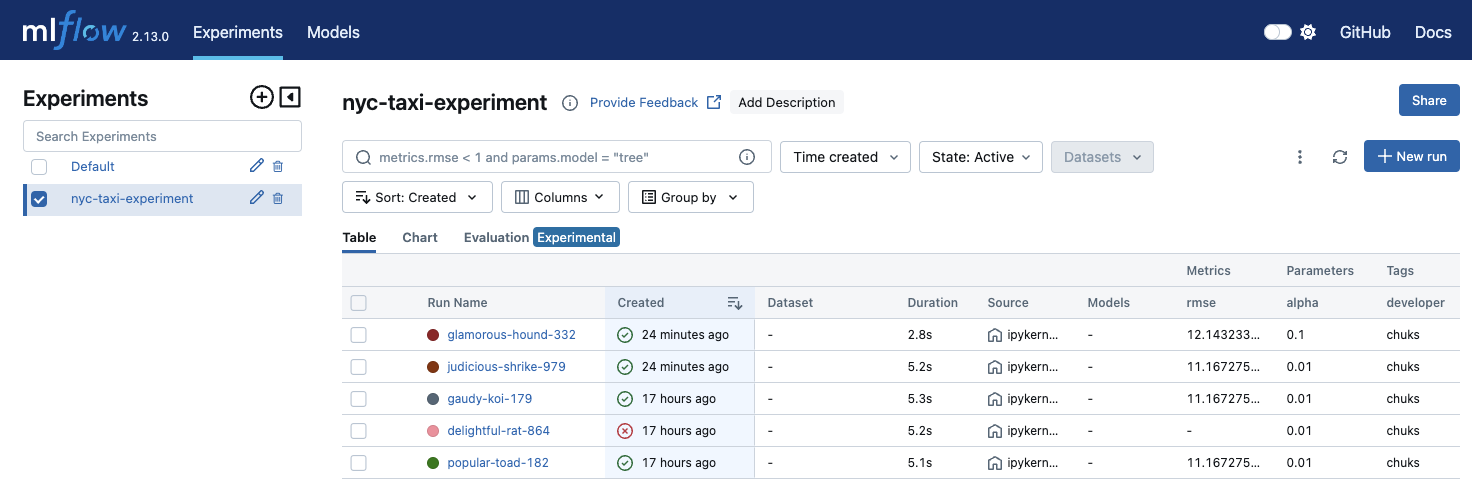
\includegraphics[width=\textwidth]{Images/mlflow-experiment-interface.png}
	\caption{MLflow Experiment Interface}
	\label{fig:3}
\end{figure}
\FloatBarrier

The updated notebook with experiment tracking using MLflow and logged predictions in MLflow UI is shown in this \href{https://github.com/chuksoo/mlops-zoomcamp-2024/blob/main/02%20-%20Experiment%20Tracking/duration-prediction.ipynb}{notebook for experiment tracking with mlflow}.

\section{Machine Learning Lifecycle}
 \begin{funfact}[frametitle=\facttitlep{Fun Fact}{MLOps cycle}]
The Machine Learning lifecycle refers to the multiple steps that are needed to build and maintain a machine learning model.
\end{funfact}

In Machine Learning Lifecycle,  we train some model, we tuned the hyperparameters, we evaluated the model and then logged some metrics, hyperparameters and other information needed to mlflow.  Once we finish with this experiment tracking stage, it means that we are happy with the model. Then we can start thinking of saving this model and have some kind of versioning. After that, we would like to deploy the model. We may realize that the model needs to be updated in order to scale. Finally, once we deploy the model, the prediction monitoring stage starts.

\begin{figure}[h]
	\centering
	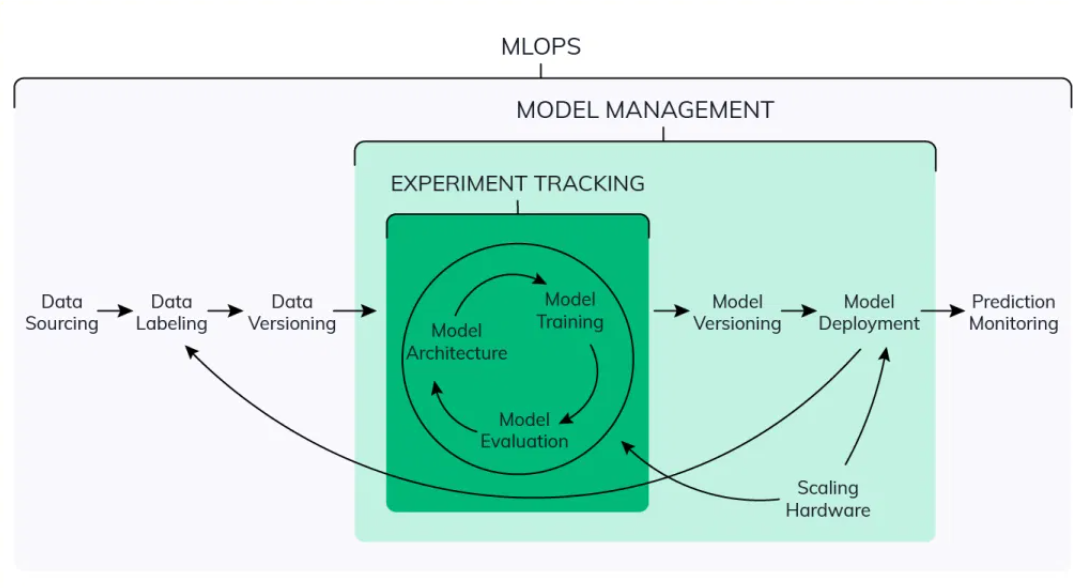
\includegraphics[width=\textwidth]{Images/neptune-mlops.png}
	\caption{MLOps cycle and machine learning experiment tracking}
	\label{fig:4}
\end{figure}
%\FloatBarrier

\subsection{Logging models in MLflow}
Two options :
\begin{itemize}[noitemsep, topsep=0pt]
\item Log model as an artifact
\begin{lstlisting}[language=python, numbers=none]
mlflow.log_artifact("<mymodel>", artifact_path="models/")
\end{lstlisting}
\item Log model using the method ``log\_model''
\begin{lstlisting}[language=python, numbers=none]
mlflow.<framework>.log_model(model, artifact_path="models/")
\end{lstlisting}
\end{itemize}

\subsection{Model Management}
Model management is a critical aspect of the machine learning lifecycle, encompassing the processes and tools used to effectively organize, version, and track machine learning models. Effective model management ensures that models can be deployed, monitored, and updated seamlessly, maintaining their performance and relevance over time. The main components of model management:

\subsubsection*{1. Versioning}
\begin{itemize}[noitemsep, topsep=0pt]
    \item \textbf{Importance:} Versioning allows data scientists to keep track of different iterations of a model, ensuring that they can reproduce results and compare performance across versions.
    \item \textbf{Tools:} Tools like MLflow, DVC, and Git provide functionalities to version models, track changes, and manage model metadata.
\end{itemize}

\subsubsection*{2. Deployment}
\begin{itemize}[noitemsep, topsep=0pt]
    \item \textbf{Purpose:} Deployment involves taking a trained model and making it available for inference in a production environment.
    \item \textbf{Methods:} Models can be deployed as a python function, in a docker container, as an APIs, embedded in applications, as a batch job in Apache Spark or integrated into data pipelines. Platforms like Kubernetes, AWS SageMaker, and Azure ML facilitate seamless deployment.
\end{itemize}

\subsubsection*{3. Monitoring}
\begin{itemize}[noitemsep, topsep=0pt]
    \item \textbf{Need:} Continuous monitoring of models in production is essential to ensure they perform as expected and to detect any performance degradation or data drift.
    \item \textbf{Metrics:} Key metrics to monitor include accuracy, latency, throughput, and error rates. Tools like Prometheus, Grafana, and custom logging solutions can be used for monitoring.
\end{itemize}

\subsubsection*{4. Retraining}
\begin{itemize}[noitemsep, topsep=0pt]
    \item \textbf{Process:} As new data becomes available, models may need to be retrained to maintain their performance.
    \item \textbf{Automation:} Automated retraining pipelines can be set up to periodically retrain models, incorporating the latest data and ensuring that the model remains up-to-date.
\end{itemize}

\subsubsection*{5. Governance and Compliance}
\begin{itemize}[noitemsep, topsep=0pt]
    \item \textbf{Compliance:} Ensuring that models comply with regulatory standards and organizational policies is crucial, especially in industries like finance and healthcare.
    \item \textbf{Documentation:} Proper documentation and audit trails are necessary for compliance and to provide transparency into how models are developed and used.
\end{itemize}

\subsubsection*{6. Collaboration}
\begin{itemize}[noitemsep, topsep=0pt]
    \item \textbf{Teamwork:} Effective model management facilitates collaboration among data scientists, engineers, and business stakeholders.
    \item \textbf{Tools:} Collaborative tools like Jupyter Notebooks, GitHub, and MLflow allow teams to share code, experiments, and insights.
\end{itemize}

\subsection*{Benefits of Effective Model Management}
\begin{itemize}[noitemsep, topsep=0pt]
    \item \textbf{Reproducibility:} Ensures that models can be consistently reproduced, which is crucial for validation and debugging.
    \item \textbf{Scalability:} Facilitates the scaling of machine learning efforts across an organization.
    \item \textbf{Efficiency:} Streamlines the deployment and monitoring processes, reducing time to market for new models.
    \item \textbf{Compliance:} Helps maintain compliance with legal and regulatory requirements.
\end{itemize}

In summary, model management is essential for maintaining the lifecycle of machine learning models, from development through deployment and monitoring, ensuring they continue to deliver value and perform optimally in production environments.

\subsection{Model Registry in Machine Learning}

    \begin{mathaside}[frametitle=\mathtitle{Why Model \color{firebrick}{registry}}]
            Model registry is an essential tool for managing the lifecycle of machine learning models, ensuring that they are well-organized, reproducible, and efficiently deployable, while enhancing collaboration and compliance within an organization.
    \end{mathaside}

A model registry is a centralized repository that stores and manages machine learning models. It plays a crucial role in the machine learning lifecycle by providing a systematic way to organize, version, and track models. The key components and benefits of a model registry:

\textbf{1. Versioning}
\begin{itemize}[noitemsep, topsep=0pt]
    \item \textbf{Purpose:} Keeps track of different iterations and versions of a model.
    \item \textbf{Functionality:} Allows comparison of model performance over time and ensures reproducibility.
\end{itemize}

\textbf{2. Metadata Management}
\begin{itemize}[noitemsep, topsep=0pt]
    \item \textbf{Purpose:} Stores important information about models, such as hyperparameters, training data, and evaluation metrics.
    \item \textbf{Functionality:} Facilitates model auditability and governance.
\end{itemize}

\textbf{3. Lifecycle Management}
\begin{itemize}[noitemsep, topsep=0pt]
    \item \textbf{Purpose:} Manages the lifecycle of models from development to deployment and monitoring.
    \item \textbf{Functionality:} Ensures smooth transitions between different stages of the model lifecycle.
\end{itemize}

\textbf{4. Access Control}
\begin{itemize}[noitemsep, topsep=0pt]
    \item \textbf{Purpose:} Defines who can access and modify models in the registry.
    \item \textbf{Functionality:} Enhances security and ensures that only authorized users can make changes.
\end{itemize}

\textbf{5. Deployment Integration}
\begin{itemize}[noitemsep, topsep=0pt]
    \item \textbf{Purpose:} Facilitates the deployment of models to production environments.
    \item \textbf{Functionality:} Provides integration with deployment tools and platforms for seamless model serving.
\end{itemize}

As we continue to generate more models, we need a model registry consisting of a tracking server to keep track of the models. Once you've decided that some of the model are ready for production, you then register the model into the mlflow model registry. Within the model registry, we have a staging , production and archive area for the models. In the model registry, all the models that are ready for production are stored here. 

\begin{figure}[h]
	\centering
	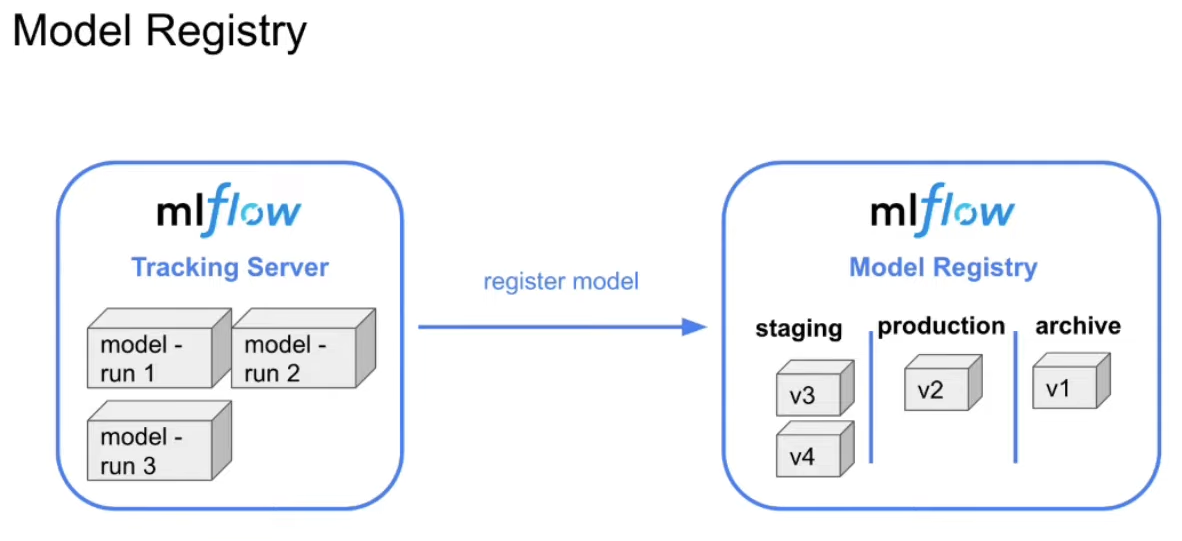
\includegraphics[width=\textwidth]{Images/model registry.png}
	\caption{Model Registry}
	\label{fig:5}
\end{figure}
\FloatBarrier

The MLOps Engineer can look at the models in the registry, inspect their hyperparameters, the size of the model and so on. He can then decide to move the models between the different stages. The model that is ready for production can be assigned to ``staging'', the current model that is used in production can be assigned to the ``production'' stage, and some of the models can be archived in the ``archived'' stage. The archived models can be retrieved from the archived stage and move them back to production if we want to roll back some deployments. The model registry is not deploying any model, it just lists the models that are production ready and the stages are just labels assigned to the model. The model registry will need to be complemented with some CI/CD code in order to do the actual deployment of the models. 

    \begin{mathaside}[frametitle=\mathtitle{Using \color{firebrick}{MLflowClient}}]
           \texttt{mlflow.client} is a module in MLflow that provides a way to interact programmatically with an MLflow tracking server. The primary class in this module is MlflowClient, which provides a comprehensive API for managing experiments, managing runs, models, logging artifacts, and interacting with model registry. 
    \end{mathaside}

\subsection{Interacting Programmatically with MLflowClient}
The \texttt{mlflow.client} module is useful for advanced use cases where you need programmatic control over MLflow entities, especially in production environments where automated workflows and integrations are required.

Here's a basic example demonstrating how to use \texttt{MlflowClient}:

\begin{lstlisting}[language=Python, caption=Example Usage of \texttt{MlflowClient}, label=code:example]
import mlflow
from mlflow.tracking import MlflowClient

# Initialize the client
client = MlflowClient()

# Create an experiment
experiment_id = client.create_experiment("My New Experiment")

# Start a new run in the experiment
run = client.create_run(experiment_id)
run_id = run.info.run_id

# Log parameters, metrics, and tags
client.log_param(run_id, "param1", 5)
client.log_metric(run_id, "metric1", 0.89)
client.set_tag(run_id, "tag1", "value1")

# Log an artifact (a file)
with open("output.txt", "w") as f:
    f.write("Hello, world!")
client.log_artifact(run_id, "output.txt")

# End the run
client.set_terminated(run_id)

# Get information about the run
run_info = client.get_run(run_id)
print(run_info)
\end{lstlisting}

\subsubsection{Key Methods of \texttt{MlflowClient}}

\subsubsection*{1. Experiment Management}
\begin{itemize}
    \item \texttt{create\_experiment(name, artifact\_location=None, tags=None)}: Creates a new experiment.
    \item \texttt{get\_experiment(experiment\_id)}: Retrieves an experiment by ID.
    \item \texttt{delete\_experiment(experiment\_id)}: Deletes an experiment.
\end{itemize}

\subsubsection*{2. Run Management}
\begin{itemize}
    \item \texttt{create\_run(experiment\_id, start\_time=None, tags=None)}: Starts a new run.
    \item \texttt{log\_param(run\_id, key, value)}: Logs a parameter.
    \item \texttt{log\_metric(run\_id, key, value, timestamp=None, step=None)}: Logs a metric.
    \item \texttt{set\_tag(run\_id, key, value)}: Sets a tag.
    \item \texttt{log\_artifact(run\_id, local\_path, artifact\_path=None)}: Logs an artifact.
\end{itemize}

\subsubsection*{3. Model Registry Management}
\begin{itemize}
    \item \texttt{create\_registered\_model(name)}: Creates a new registered model.
    \item \texttt{create\_model\_version(name, source, run\_id, tags=None, run\_link=None, description=None)}: Creates a new model version.
    \item \texttt{transition\_model\_version\_stage(name, version, stage)}: Transitions a model version to a new stage.
\end{itemize}

\section{MLflow in Practice}
\subsection{Different scenarios for running MLflow}
Let's consider these three scenarios:
\begin{itemize}[noitemsep, topsep=0pt]
\item \textbf{\smtt{A single data scientist participating in an ML competition}}: In this scenario, having remote tracking server will be an overkill. Saving this information locally will be enough. Also, using model registry is useless since the data scientist is not deploying this model to production.
\item \textbf{\smtt{A cross-functional team with one data scientist working on an ML model}}:Here, sharing the experiment information is important. Also, using model registry will be a good idea but it can be run remotely or local host.
\item \textbf{\smtt{Multiple data scientists working on multiple ML models}}: Since multiple data scientist are working on multiple model, collaboration and sharing experiment information is very important. One data scientist can build the model, another data scientist can tune different hyperparameters to add to the model. They need a way to keep track of the models using a remote tracking server. Also, it is important to manage the lifecycle of the model since multiple people build and deploy the model hence model registry is important. 
\end{itemize}

\subsection{Things to Consider before Configuring MLflow}
There are different things to consider before configuring MLflow.
\begin{itemize}[noitemsep, topsep=0pt]
\item \textbf{Backend Store}: Where MLflow saves information about your experiement such as metadata, models etc
	\begin{itemize}[label={\ding{224}}]
		\item local filesystem
		\item SQLAlchemy compatible DB (e.g. SQLite)
	\end{itemize}
\item \textbf{Artifacts Store}: Decide where to store the artifact i.e., locally or remote
	\begin{itemize}[label={\ding{224}}]
		\item local filesystem
		\item remote (e.g.  s3 bucket)
	\end{itemize}
\item \textbf{Tracking Server}: Decide how to run tracking server
	\begin{itemize}[label={\ding{224}}]
		\item no tracking server
		\item localhost
		\item remote
	\end{itemize}
\end{itemize}

\subsection{Setting Up MLflow Tracking Server in AWS}
Assuming we have multiple data scientist working on multiple ML models. We can setup a remote tracking server on \href{https://aws.amazon.com/ec2/}{Amazon Elastic Compute Cloud (Amazon EC2)} with PostgreSQL backend using \href{https://aws.amazon.com/rds/}{Amazon Relational Databse Service (RDS)} and \href{https://aws.amazon.com/s3/}{Amazon Simple Storage Service (S3)} to store the model and artifacts. MLflow uses the backend store and artifact store for persistent runs. The PostgreSQL backend stores metadata such as parameters, metrics, and tags while the artifact store holds large files such as serialized models and config files. MLflow experiments can be explored by accessing the remote server. To run experiments using AWS, we have to configure an AWS account.

\subsubsection{Basic AWS Setup}

 \begin{itemize}
\item \textbf{Step 1}: Launch a new EC2 instance \\
For this, you can select one of the instance types that are free tier eligible. For example, we will select an Amazon Linux OS (\smtt{Amazon Linux 2 AMI (HVM) - Kernel 5.10, SSD Volume Type}) and a \smtt{t2.micro} instance type, which are free tier eligible.
\begin{figure}[h]
	\centering
	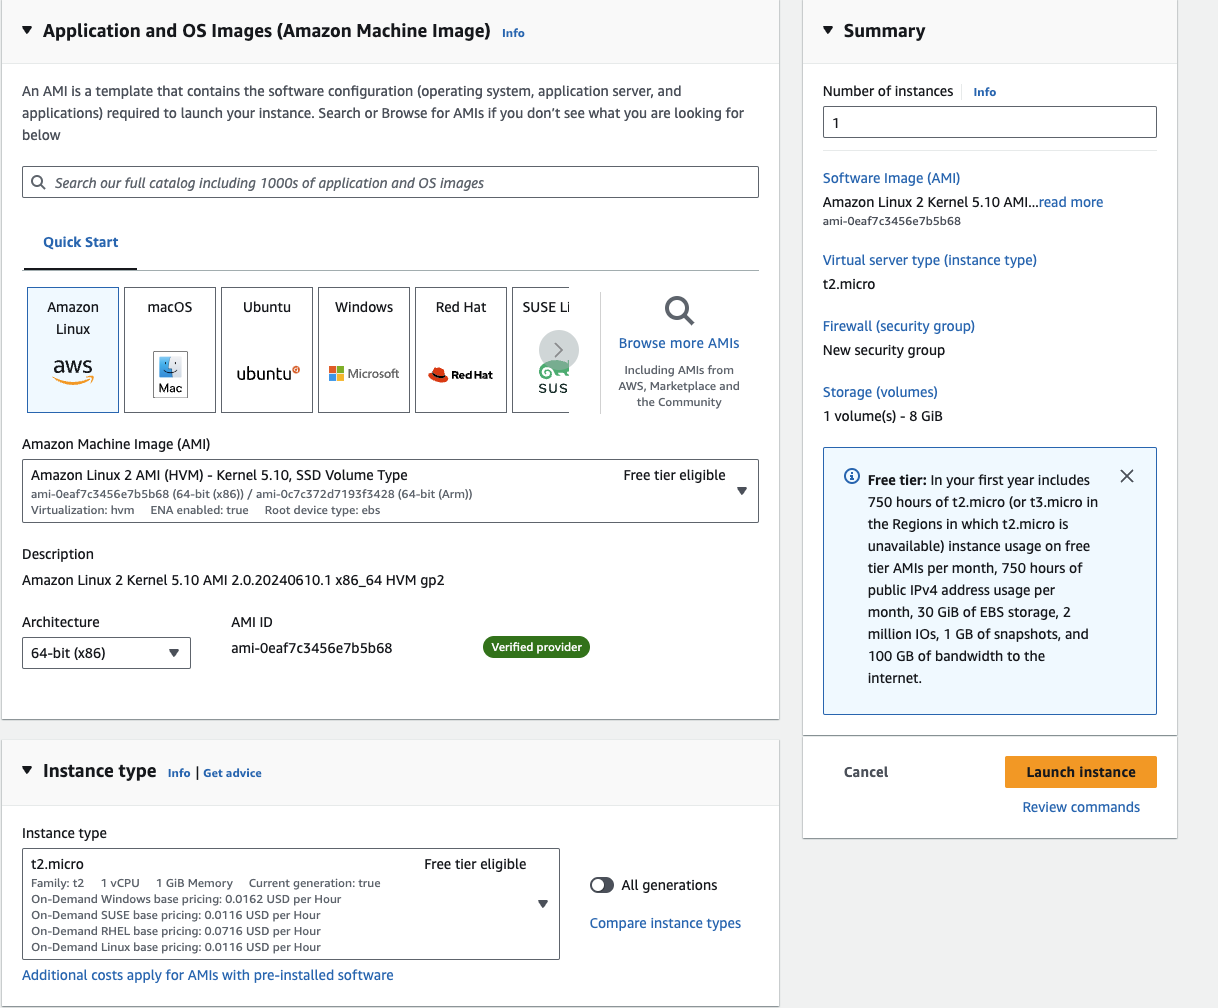
\includegraphics[width=\textwidth]{Images/EC2-setup.png}
	\caption{Application and OS Setup}
	\label{fig:6}
\end{figure}
\FloatBarrier
You'll also need to create a new key pair so later you can connect to the new instance using SSH. Click on ``Create new key pair'' and complete the details like in the image below:
\begin{figure}[h]
	\centering
	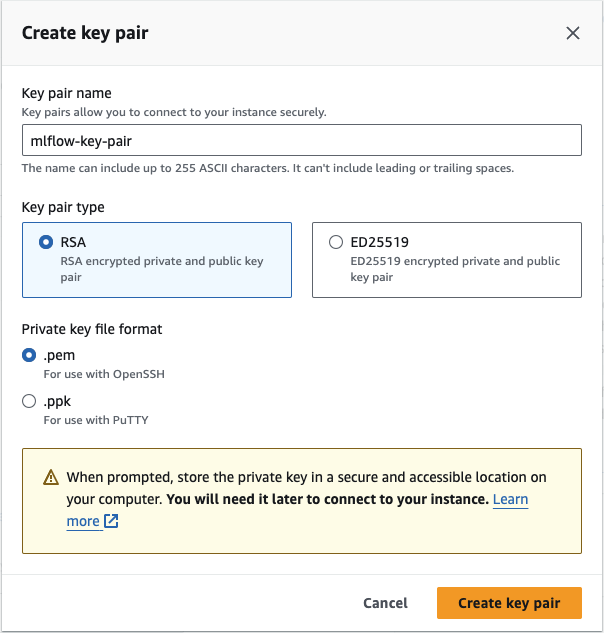
\includegraphics[width=0.65\textwidth]{Images/mlflow-key-pair.png}
	\caption{Create Key Pair}
	\label{fig:7}
\end{figure}
\FloatBarrier

Select the new key pair and then click on ``Launch Instance''.

\begin{figure}[h]
	\centering
	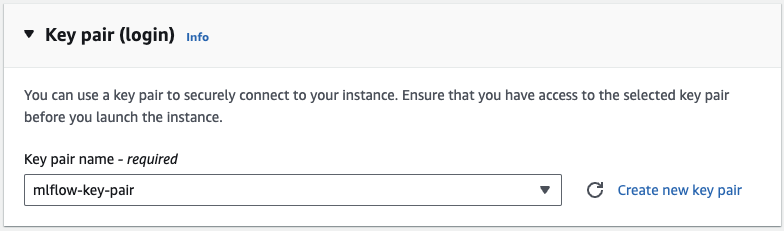
\includegraphics[width=0.65\textwidth]{Images/key-pair-setup.png}
	\caption{Select Key Pair}
	\label{fig:8}
\end{figure}
\FloatBarrier
 Leave the rest of the configuration the way it is an launch the instance.

\item \textbf{Step 2}:  Configure the security group \\
Open up the new instance and select the newly created ``Security groups'' in ``Security''. Edit security group so the EC2 instance accepts SSH (port 22) and HTTP connections (port 5000). Do this by ``Edit Inbound rules''. 
\begin{figure}[h]
	\centering
	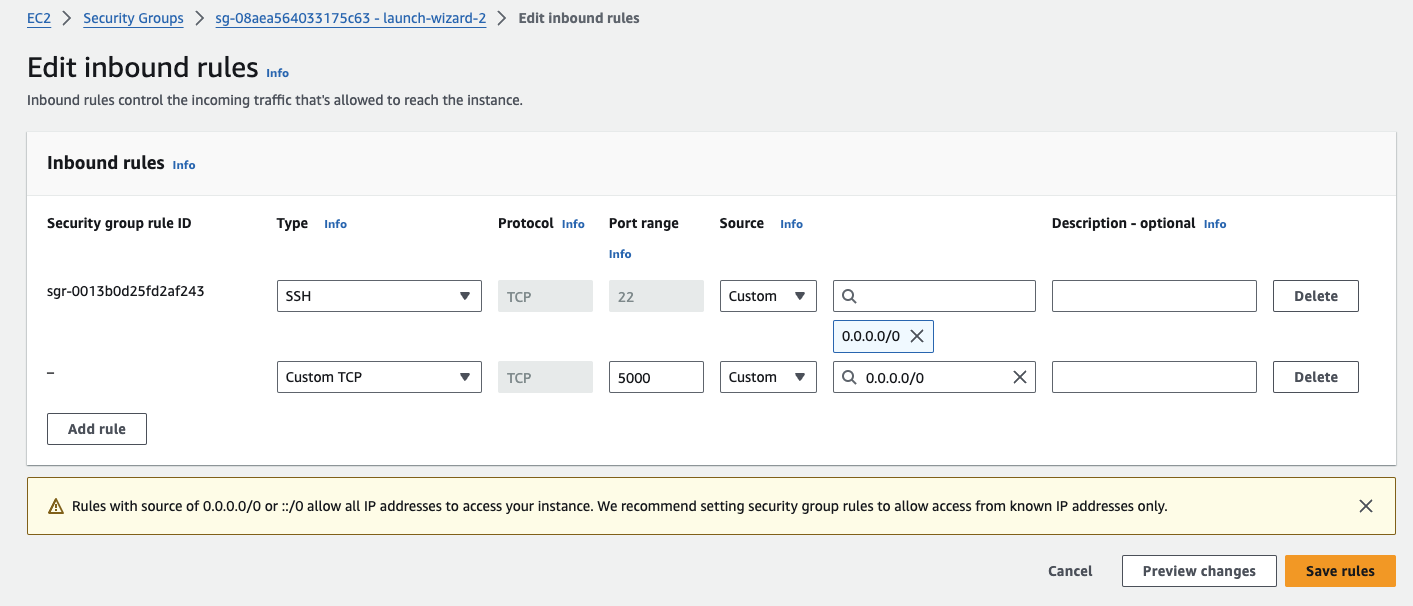
\includegraphics[width=0.65\textwidth]{Images/security-group.png}
	\caption{Security group setup}
	\label{fig:9}
\end{figure}
\FloatBarrier

\item \textbf{Step 3}: Create an S3 bucket \\
The Amazon Simple Storage Service (S3) will be used as the artifact store. Go to ``S3'' and click on ``Create bucket''. Fill in the bucket name as in the image below and leave all the other configurations with their default values.
\begin{figure}[h]
	\centering
	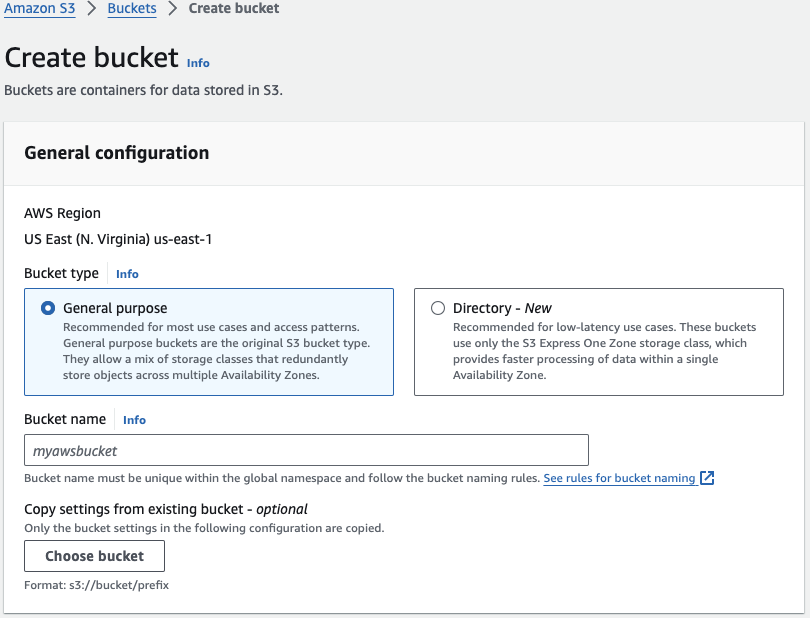
\includegraphics[width=0.65\textwidth]{Images/S3-setup.png}
	\caption{S3 bucket setup}
	\label{fig:10}
\end{figure}
\FloatBarrier

\item \textbf{Step 4}: Create a new PostgreSQL database in RDS \\
The Amazon Relational Databse Service (RDS) uses PostgreSQL engine as the backend store. Go to the RDS Console and click on ``Create database''. Make sure to select ``PostgreSQL'' engine type and the ``Free tier'' template.

\begin{figure}[h]
	\centering
	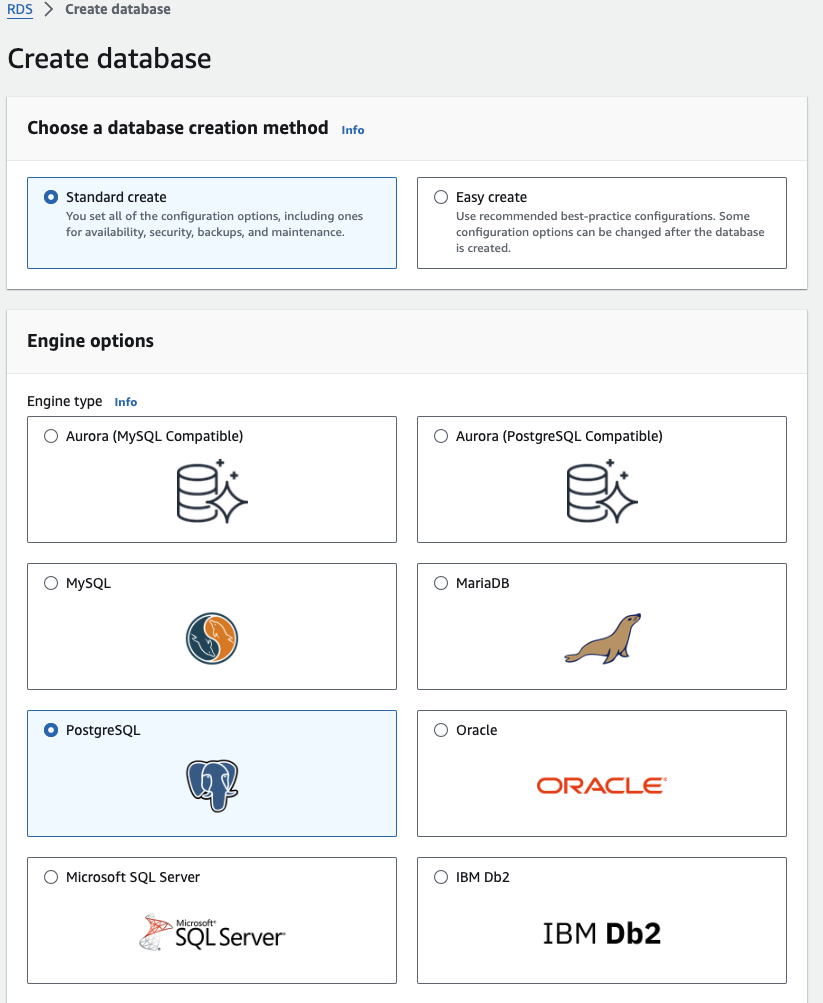
\includegraphics[width=0.5\textwidth]{Images/create-database.png}
	\caption{Create RDS Database}
	\label{fig:11}
\end{figure}
\FloatBarrier

\begin{figure}[h]
	\centering
	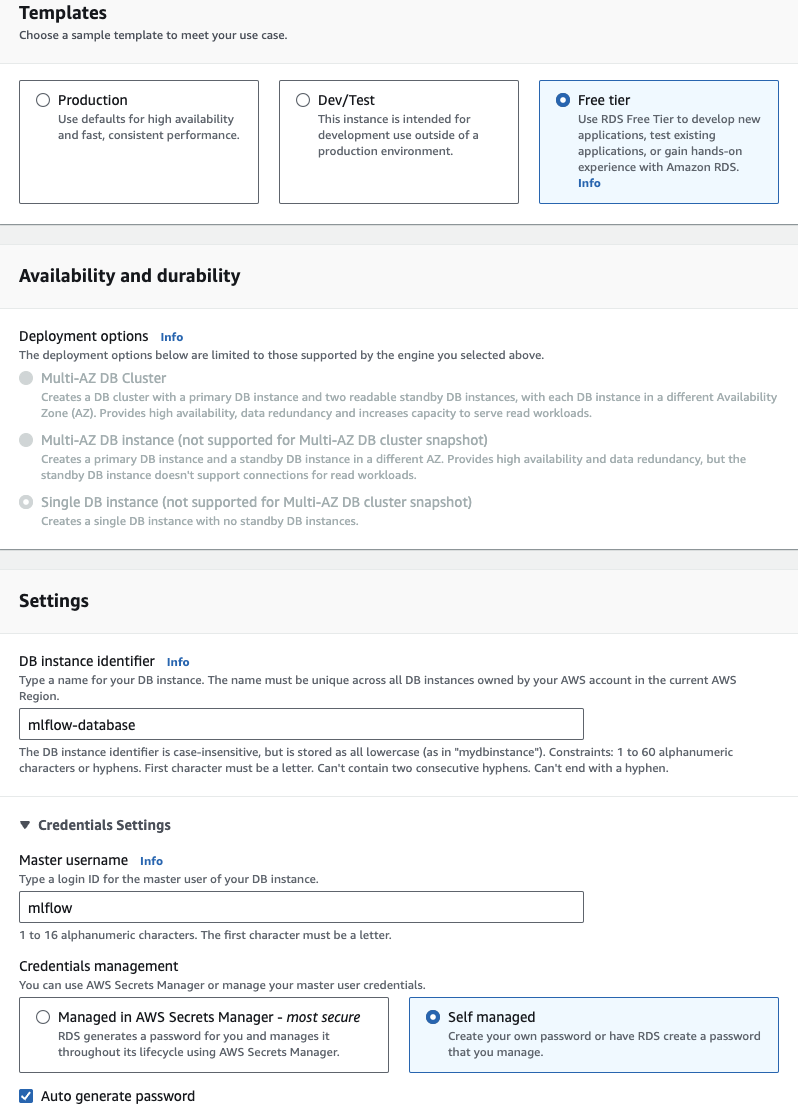
\includegraphics[width=0.5\textwidth]{Images/RDS-setup.png}
	\caption{Setup RDS username and password}
	\label{fig:12}
\end{figure}
\FloatBarrier

Select a name for your DB instance, set the master username as ``mlflow'' and tick the option ``Auto generate a password'' so Amazon RDS generate a password automatically.  Setup instance connection, use the default VPC and connectivity to the compute resource. Use default values for all the other configurations.

\begin{figure}[h]
	\centering
	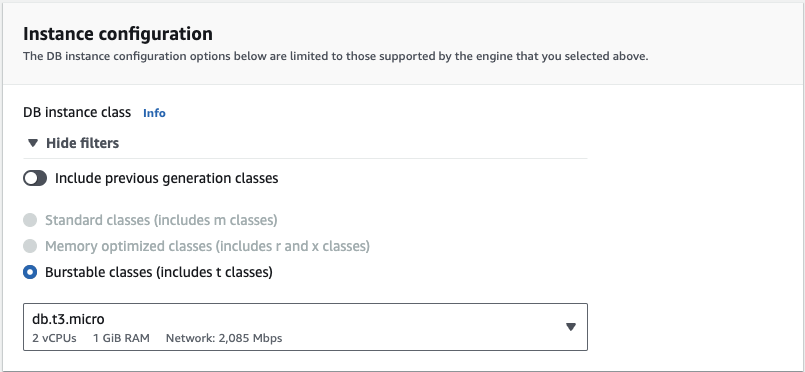
\includegraphics[width=0.5\textwidth]{Images/instance-configuration.png}
	\caption{Instance Configuration}
	\label{fig:13}
\end{figure}
\FloatBarrier

\begin{figure}[h]
	\centering
	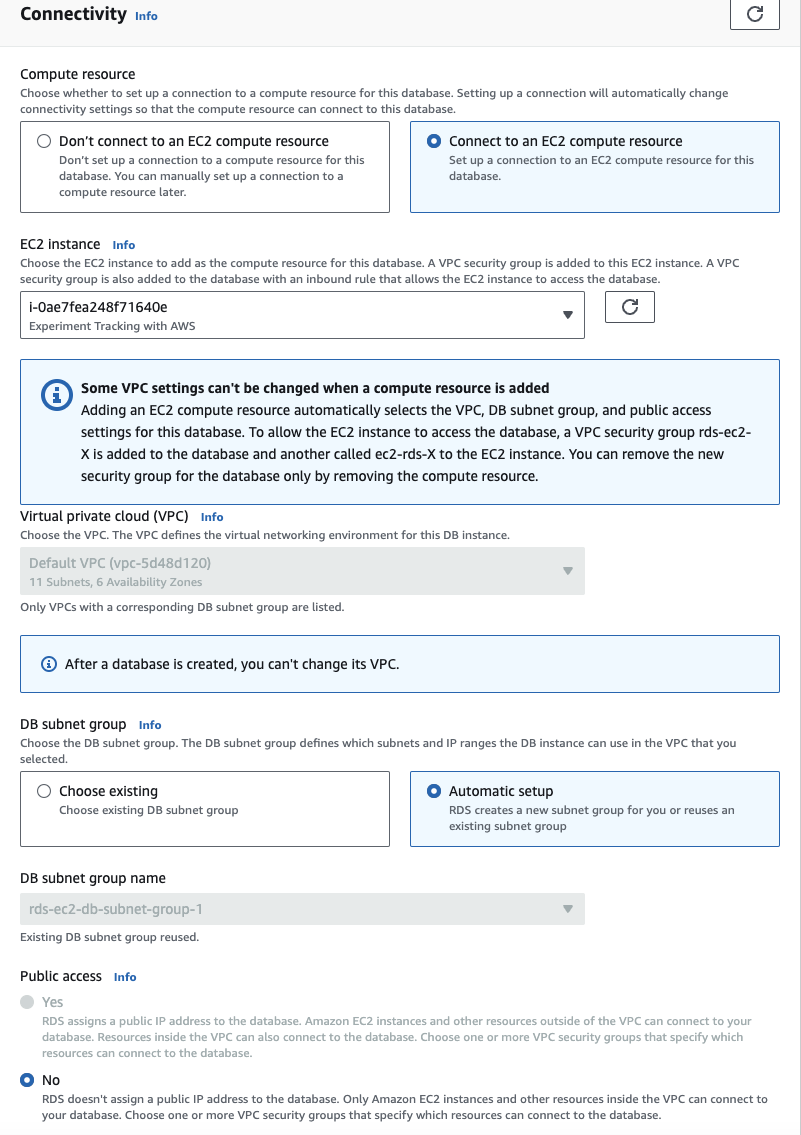
\includegraphics[width=0.5\textwidth]{Images/EC2 connectivity to DB.png}
	\caption{EC2 connectivity to DB}
	\label{fig:14}
\end{figure}
\FloatBarrier

\begin{figure}[h]
	\centering
	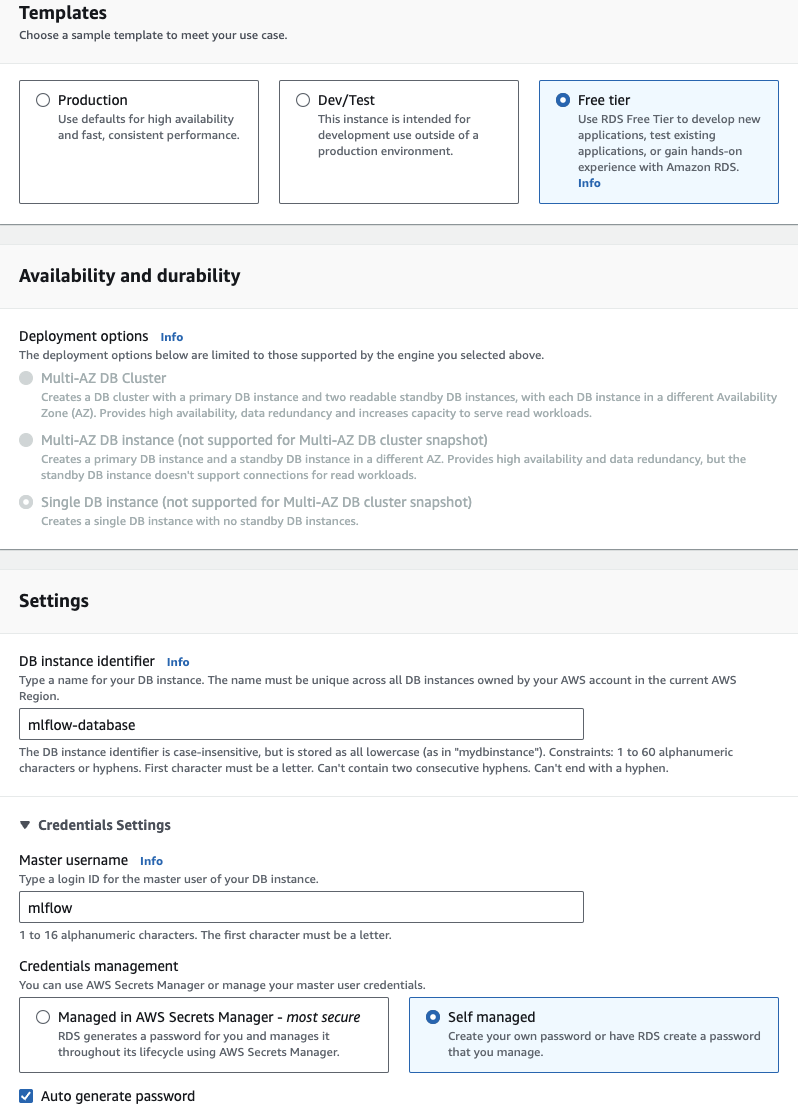
\includegraphics[width=0.5\textwidth]{Images/RDS-setup.png}
	\caption{RDS Setup}
	\label{fig:15}
\end{figure}
\FloatBarrier

Specify a database name so that RDS will create the database for you.

\begin{figure}[h]
	\centering
	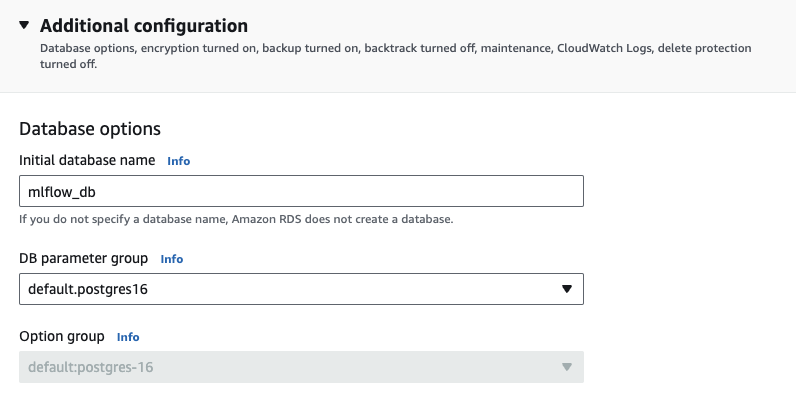
\includegraphics[width=0.5\textwidth]{Images/set-db-name.png}
	\caption{Additional configuration to set database name}
	\label{fig:16}
\end{figure}

After clicking on ``launch database'' you will be able to check the newly generated password, but take into account that the automatically generated password will be shown only once!. Take note of the master username, password, initial database name, and endpoint. 


Once the DB instance is created, go to the RDS console, select the new db and under ``Connectivity \& security'' select the VPC security group. Modify the security group by adding a new inbound rule that allows postgreSQL connections on the port 5432 from the security group of the EC2 instance. This way, the server will be able to connect to the postgres database.

\begin{figure}[h]
	\centering
	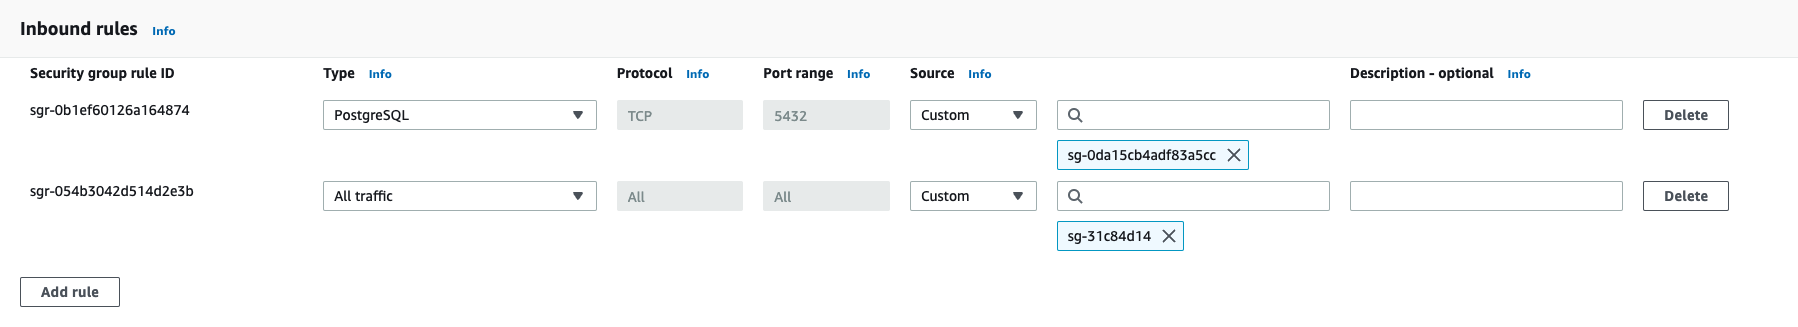
\includegraphics[width=0.65\textwidth]{Images/postgresql_inbound_rule.png}
	\caption{Edit Security Groups}
	\label{fig:17}
\end{figure}



\item \textbf{Step 5}: Connect to the EC2 instance and launch the tracking server \\
Go to the EC2 Console and find the instance launched and click on ``Connect'' and then follow the steps described in the tab ``SSH''.

Run the following commands to install the dependencies, configure the environment and launch the server:

\begin{lstlisting}[language=python, numbers=none]
sudo yum update
pip3 install mlflow boto3 psycopg2-binary
aws configure # you'll need to input your AWS credentials here
mlflow server -h 0.0.0.0 -p 5000 --backend-store-uri postgresql://DB_USER:DB_PASSWORD@DB_ENDPOINT:5432/DB_NAME --default-artifact-root s3://S3_BUCKET_NAME
\end{lstlisting}
Note: before launching the server, check that the instance can access the s3 bucket created. To do that, just run this command from the EC2 instance: \smtt{aws s3 ls}. You should see the bucket listed in the result.

\item \textbf{Step 6}: Access the remote tracking server from your local machine \\
Open a new tab on your web browser and go to this address: \smtt{http://<EC2\_PUBLIC\_DNS>:5000} (you can find the instance's public DNS by checking the details of your instance in the EC2 Console).
\end{itemize}

\section{MLflow: Benefits, limitations and alternatives}
\subsection{Remote tracking server}
The tracking server can be easily deployed to the cloud. Some of the benefits are:
\begin{itemize}[noitemsep, topsep=0pt]
\item Shared experiments with other data scientist
\item Collaborate with others to build and deploy models
\item Give more visibility of the data science efforts
\end{itemize}

\subsection{Issues with running a remote (shared) MLflow server}
Some issues can arise when running a remote MLflow server. They include:
\begin{itemize}[noitemsep, topsep=0pt]
\item Security
	\begin{itemize}[label={\ding{224}}]
	\item Restrict access to the server (e.g. access through VPN)
	\end{itemize}
\item Scalability
	\begin{itemize}[label={\ding{224}}]
	\item Check \href{https://aws.amazon.com/blogs/machine-learning/managing-your-machine-learning-lifecycle-with-mlflow-and-amazon-sagemaker/}{Deploy MLflow on AWS Fargate}
	\item Check \href{https://www.slideshare.net/databricks/mlflow-at-company-scale-239587085}{MLflow at Company Scale}
	\end{itemize}
\item Isolation
	\begin{itemize}[label={\ding{224}}]
	\item Define standard for naming experiments, modles, and a set of default tags
	\item Restrict access to artifacts (e.g. use s3 buckets living in different AWS accounts)
	\end{itemize}
\end{itemize}

\begin{figure}[h]
	\centering
	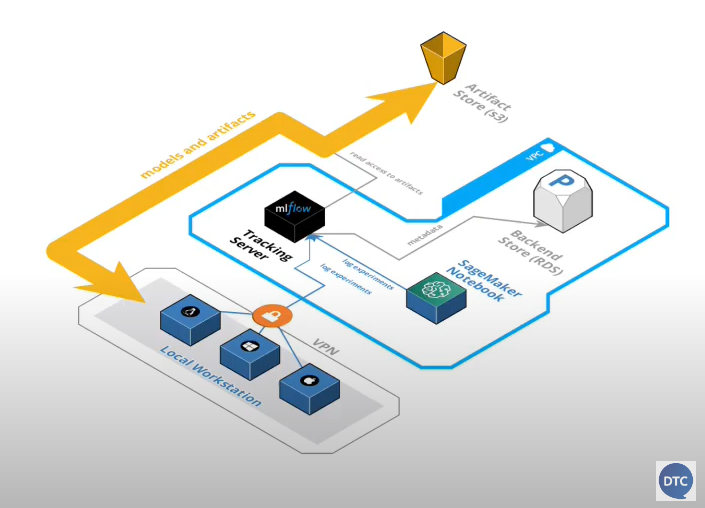
\includegraphics[width=\textwidth]{Images/remote tracking-mlflow.png}
	\caption{Remote Tracking Server with MLflow}
	\label{fig:6}
\end{figure}
\FloatBarrier

\subsection{MLflow limitations (and when not to use it)}
There are some limitations for MLflow. For example:
\begin{itemize}[noitemsep, topsep=0pt]
\item \textbf{Authetication \& Users:} The open source version of MLflow doesn't provide any sort of authetication.
\item \textbf{Data versioning:} To ensure full reproducibility, we need to version the data used to train the model. MLflow doesn't provide a built-in solution for that but there are a few ways to deal with this limitation.
\item \textbf{Model/Data Monitoring \& Alerting:} This is outside the scope of MLflow and currently there are more suitable tools for doing this.
\end{itemize}

There are some paid alternatives to MLflow including Neptune.ai, Comet, Weight \& Biases and many more. 

%--------------- Chapter 3: Orchestration and ML Pipelines -----------%
\chapter{Orchestration and ML Pipelines} \label{ch:3}
\section{Introduction: ML pipelines and Mage}
\subsection{Operationalizing ML models}
 \begin{funfact}[frametitle=\facttitlep{Fun Fact}{Operationalizing ML models}]
Operationalizing ML models involves moving them from development to production to drive business value
\end{funfact}

To operationalize ML models, we take the following steps:
\begin{itemize}[noitemsep, topsep=0pt]
\item \textbf{\smtt{Preparing the model for deployment}} involves optimizing performance, ensuring it handles real-world data, and packaging it for integration into existing systems.
\item \textbf{\smtt{Deploying the model}} involves moving it from development to production, making it accessible to users and applications.
\item Once deployed, models must be \textbf{\smtt{continuously monitored for accuracy and reliability,}} and may need retraining on new data and updates to maintain effectiveness.
\item \textbf{\smtt{Integrating operationalized model into existing workflows, applications, and decision-making processes}} to drive business impact.
\end{itemize}
Effective operationalization enables organizations to move beyond experimentation and drive tangible value from ML at scale, powering intelligent applications that personalize the customer experience and creates real business value.

\subsection{Why we need to operationalize ML}
\begin{itemize}[noitemsep, topsep=0pt]
\item \textbf{Productivity} - MLOps fosters collaboration between data scientists, ML engineers, and DevOps teams by providing a unified environment for experiment tracking, feature engineering, model management, and deployment. This breaks down silos and accelerates the entire machine learning lifecycle.
\item \textbf{Reliability} - MLOps ensures high-quality, reliable models in production through clean datasets, proper testing, validation, CI/CD practices, monitoring, and governance.
\item \textbf{Reproducibility} - MLOps enables reproducibility and compliance by versioning datasets, code, and models, providing transparency and auditability to ensure adherence to policies and regulations.
\item \textbf{Time-to-value} - MLOps streamlines the ML lifecycle, enabling organizations to successfully deploy more projects to production and derive tangible business value and ROI from AI/ML investments at scale.
\end{itemize}

\subsection{How Mage helps MLOps}
\begin{itemize}[noitemsep, topsep=0pt]
\item \textbf{Data preparation} - Mage offers features to build, run, and manage data pipelines for data transformation and integration, including pipeline orchestration, notebook environments, data integrations, and streaming pipelines for real-time data.
\item \textbf{Training and deployment} - Mage helps prepare data, train machine learning models, and deploy them with accessible API endpoints.
\item \textbf{Standardize complex processes} - Mage simplifies MLOps by providing a unified platform for data pipelining, model development, deployment, versioning, CI/CD, and maintenance, allowing developers to focus on model creation while improving efficiency and collaboration.
\end{itemize}

\subsection{Project setup for Mage}
Clone the following respository containing the complete code for this module:
\begin{lstlisting}[language=python, numbers=none]
git clone https://github.com/mage-ai/mlops.git
\end{lstlisting}

Change directory into the cloned repo:
\begin{lstlisting}[language=python, numbers=none]
cd mlops
\end{lstlisting}

Launch Mage and the database service (PostgreSQL):
\begin{lstlisting}[language=python, numbers=none]
./scripts/start.sh
\end{lstlisting}

If you don't have bash in your enviroment, modify the following command and run it:
\begin{lstlisting}[language=python, numbers=none]
PROJECT_NAME=mlops \
    MAGE_CODE_PATH=/home/src \
    SMTP_EMAIL=$SMTP_EMAIL \
    SMTP_PASSWORD=$SMTP_PASSWORD \
    docker compose up
\end{lstlisting}

The subproject that contains all the pipelines and code is named \texttt{unit\_3\_observability}

\section{Data preparation: ETL and Feature Engineering}
\section{Training: sklearn models and XGBoost}
\section{Observability: Monitoring and Alerting}
\section{Triggering: Inference and Retraining}
\section{Deploying: Running operations in Production}

%--------------- Chapter 4: Deployment -----------%
\chapter{Deployment} \label{ch:4}
\section{Model Deployment}
\subsection{Three ways of deploying models}
 \begin{funfact}[frametitle=\facttitlep{Fun Fact}{Deploying ML models}]
Deploying machine learning model models is an iterative process that often involves multiple rounds of training, testing, and validating before the model is ready for production.
\end{funfact}

Deploying a model means that other application can get predictions from our model. There are three modes of deployment namely \textbf{online} deployment, \textbf{offline} or batch deployment, and \textbf{streaming}.

First, we need to ask ourselves if we need to have predictions immediately or it can wait a little bit for an hour, a day or a week. If it can wait for a little bit, then we go for batch deployment. i.e., the model is not running all the time and we just apply our model to new data regularly. In online deployment, the model is up and running all the time and is always available. Two variant of online deployment is deployment as a web service and deployment via streaming. In web service deployment, we send HTTP requests and the service sends out prediction. In streaming, there is an ``events model service'' listening for events on the stream and reacting to this event. 

\subsection{Web services: Introduction to Flask}
    \begin{mathaside}[frametitle=\mathtitle{Web \color{firebrick}{Service}}]
       A  \texttt{web service} is a method for communicating between two devices over a network using some protocols.
    \end{mathaside}
Assuming we want to use our model inside a \texttt{churn service} in order to make some predictions. The \texttt{marketing service} will communicate with our churn service by sending some request and getting a response. This can be done using a web service. In \textbf{web service}, a user sends a request in the form of a query, then the web service sends back a response to the user with the result.  In \textbf{Fig. \ref{fig:7}}, we have a notebook that was used to train the churn model. The model is saved to file. We can load this model from a different process or web service called the \texttt{churn service}. If the \texttt{marketing service} wants to identify if the user will churn, they send a request to the \texttt{churn service} with information about the user then they get back the predictions and based on these predictions, the marketing service can decide whether they want to send a promotional email with say 25\% discount to prevent churn.  

\begin{figure}[h]
	\centering
	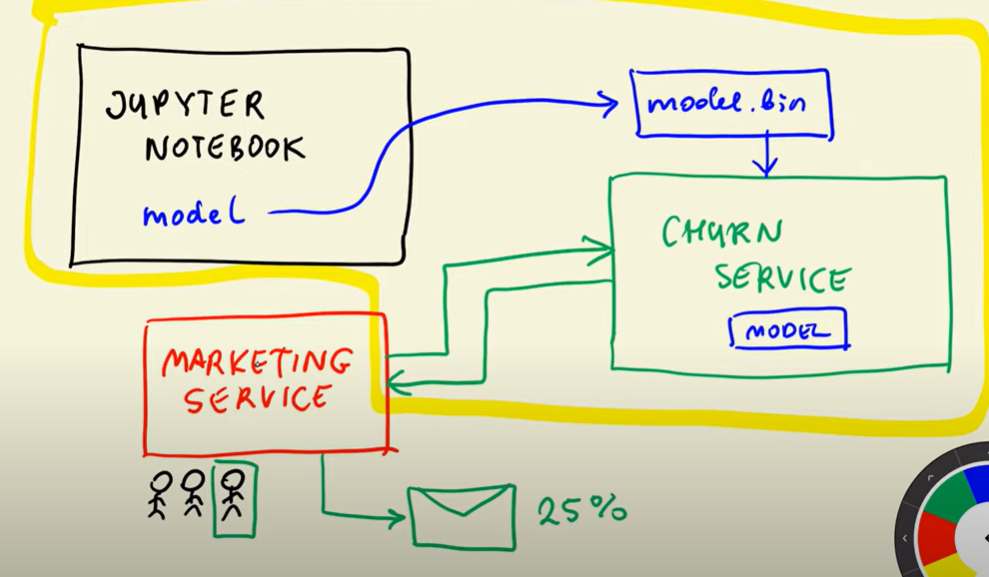
\includegraphics[width=\textwidth]{Images/model-serving.png}
	\caption{Serving Churn Model}
	\label{fig:7}
\end{figure}
\FloatBarrier

To do this, we put the model inside a web service using \textbf{flask}, which is a framework for creating web services in python, then we isolate dependencies for this service so they don't interfere with other services on ur machine by creating a special environment for python dependencies using \textbf{Pipenv}. Then we add another layer with system dependencies using \textbf{Docker}, and then finally we deploy the container containing this model to the cloud using \textbf{AWS Elastic Beanstalk}.

\begin{figure}[h]
	\centering
	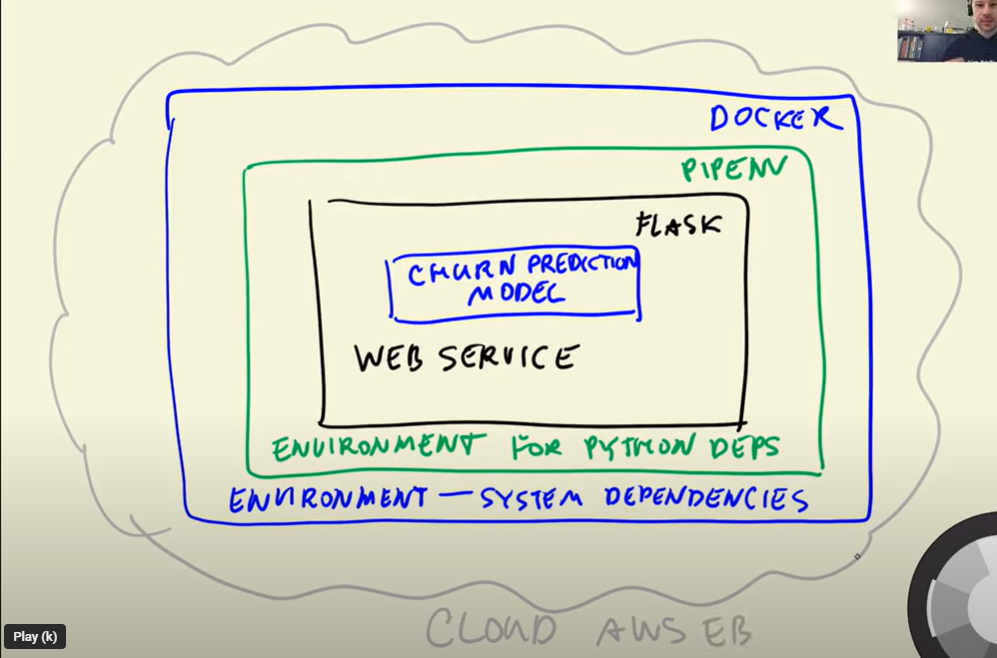
\includegraphics[width=\textwidth]{Images/layers-to-deployment.png}
	\caption{Layers to deployment}
	\label{fig:8}
\end{figure}
\FloatBarrier

To deploy a model, we turn our notebook to Python script called \texttt{train.py} where we save the model as a pickle file. Then using our \texttt{predict.py}, we can load the model and make prediction. 

There are some methods in web services we can use it to satisfy our problems. Here below we would list some.
\begin{itemize}[noitemsep, topsep=0pt]
 \item \texttt{GET}: GET is a method used to retrieve files, For example when we are searching for a cat image in google we are actually requesting cat images with GET method.
 \item \texttt{POST}: POST is the second common method used in web services. For example in a sign up process, when we are submiting our name, username, passwords, etc we are posting our data to a server that is using the web service. (Note that there is no specification where the data goes)
 \item \texttt{PUT}: PUT is same as POST but we are specifying where the data is going to.
 \item \texttt{DELETE}: DELETE is a method that is used to request to delete some data from the server.
\end{itemize}

We can create a simple service using flask that pings and send a response back. To do that, we create a \texttt{ping.py} file containing:
\begin{lstlisting}[language=python, numbers=none]
from flask import Flask

app = Flask('ping')

@app.route('/ping', methods=['GET'])
def ping():
    return "PONG"

if __name__ == '__main__':
    app.run(debug=True, host='0.0.0.0', port=9696)
\end{lstlisting}

We start by installing and importing flask
\begin{lstlisting}[language=python, numbers=none]
from flask import Flask
\end{lstlisting}

We create a flask app
\begin{lstlisting}[language=python, numbers=none]
app = Flask('ping')
\end{lstlisting}

and then add a decorator, which is a way to add some extra functionality to our functions. This extra functionality will allow us turn the function into a web service. We specify the address the 'ping' will live in, and the method to access this route. 
\begin{lstlisting}[language=python, numbers=none]
@app.route('/ping', methods=['GET'])
\end{lstlisting}

We run the app in debug mode and specify the host to run on.
\begin{lstlisting}[language=python, numbers=none]
if __name__ == '__main__':
    app.run(debug=True, host='0.0.0.0', port=9696)
\end{lstlisting}

We get the following output when it runs:
\begin{figure}[h]
	\centering
	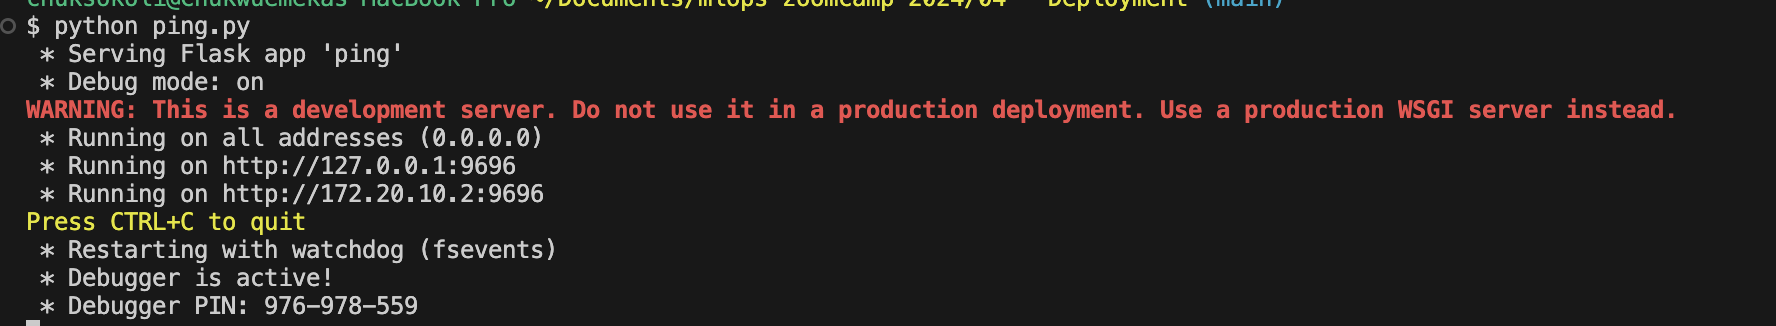
\includegraphics[width=\textwidth]{Images/ping.png}
	\caption{Ping result}
	\label{fig:9}
\end{figure}
\FloatBarrier
To test it, open your browser and search \smtt{localhost:9696/ping}, You'll see that the 'PONG' string is received. Congrats You've made a simple web server.

\subsection{Serving the Churn Model with Flask}
In serving the churn model with flask, we want the model to be available at \smtt{/predict} in the \texttt{churn service}. The \texttt{marketing service} will send the \texttt{churn service} with information about the customers, and then we reply them with the probability of churning. The \texttt{churn service} also sends a promotional email to the customer with 25\% discount. To make the web service predict the churn value for each customer, we need to first load the previous saved model and use a prediction function in a special route.
\begin{figure}[h]
	\centering
	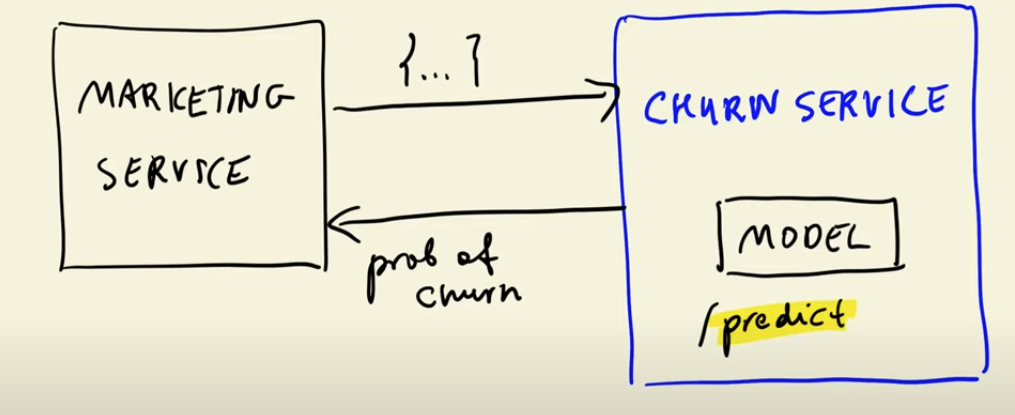
\includegraphics[width=\textwidth]{Images/deploy-flask.png}
	\caption{Ping result}
	\label{fig:10}
\end{figure}
\FloatBarrier
\begin{itemize}[noitemsep, topsep=0pt]
\item To load the previous saved model, we create a \texttt{predict.py} file that loads the model
\begin{lstlisting}[language=python, numbers=none]
# Load the model
import pickle
from flask import Flask
from flask import request
from flask import jsonify

model_file = 'model_C=1.0.bin'

# load the model
with open(model_file, 'rb') as f_in: # read binary file
    dv, model = pickle.load(f_in)    # load() loads the file 
\end{lstlisting}
\item A function to predict a value for a customer
\begin{lstlisting}[language=python, numbers=none]
def predict_single(customer, dv, model):
    X = dv.transform([customer])  # one-hot encoding to the data 
    y_pred = model.predict_proba(X)[:, 1]
    return y_pred[0]
\end{lstlisting}
\item Then the function used to create the web service that makes prediction and sends an email to the customer.
\begin{lstlisting}[language=python, numbers=none]
app = Flask('churn') # name of the app
@app.route('/predict', methods=['POST'])  # in order to send the customer information we need to post its data.
def predict():
    customer = request.get_json()  # web services work best with json frame
    prediction = predict_single(customer, dv, model)
    churn = prediction >= 0.5

    result = {
        'churn_probability': float(prediction),  # cast numpy float type to python native float type
        'churn': bool(churn),  # casting the value using bool method
    }
    return jsonify(result)  # send back the data in json format to the user
\end{lstlisting}
\end{itemize}

To deploy,  the customer information in the \texttt{deploy.py} file is sent as JSON. The predict script is turned into a web service and sends a response back to the \texttt{marketing service} with predictions as JSON and an email to the customer likely to churn.
\begin{lstlisting}[language=python, numbers=none]

customer_id = "asdx-123d"
customer_email = "asdx-123d@yahoo.com"
customer = {
    "gender": "female",
    "seniorcitizen": 0,
    "partner": "yes",
    "dependents": "no",
    "phoneservice": "no",
    "multiplelines": "no_phone_service",
    "internetservice": "dsl",
    "onlinesecurity": "no",
    "onlinebackup": "yes",
    "deviceprotection": "no",
    "techsupport": "no",
    "streamingtv": "no",
    "streamingmovies": "no",
    "contract": "two_year",
    "paperlessbilling": "yes",
    "paymentmethod": "electronic_check",
    "tenure": 10,
    "monthlycharges": 29.85,
    "totalcharges": (2 * 29.85)
}
# Making requests
import requests
url = "http://localhost:9696/predict"
response = requests.post(url, json=customer).json()
print(response)

if response["churn"]:
    print(f"Sending email to {customer_id} with email:", {customer_email})
else:
    print(f"Customer {customer_id} will not churn")
\end{lstlisting}

You can run the prediction app using:
\begin{lstlisting}[language=python, numbers=none]
python predict.py
\end{lstlisting}
When you run the app, you will see a warning that it is not a WGSI server and not suitable for production environments. To fix this issue and run this as a production server there are plenty of ways available. One way to create a WSGI server is to use gunicorn. To install it use the command 
\begin{lstlisting}[language=python, numbers=none]
pip install gunicorn
\end{lstlisting}
And to run the WGSI server you can simply run it with the command 
\begin{lstlisting}[language=python, numbers=none]
gunicorn --bind 0.0.0.0:9696 predict:app 
\end{lstlisting}

Note that in \texttt{predict:app} the name ``predict'' is the name we set for the file containing the code \texttt{app = Flask('churn')}(for example: predict.py), You may need to change it to whatever you named your Flask app file. So far, we have been able to make a production server that predict the churn value for new customers.

\subsection{Dependencies and Environment Management: Pipenv}
Every time we're running a file from a directory we're using the executive files from a global directory. For example when we install python on our machine the executable files that are able to run our codes will go to somewhere like \smtt{\textbf{/home/username/python/bin/}} for example the pip command may go to \smtt{\textbf{/home/username/python/bin/pip}}. Sometimes the versions of libraries conflict (the project may not run or get into massive errors). For example we have an old project that uses sklearn library with the version of 0.24.1 and now we want to run it using sklearn version 1.0.0. We may get into errors because of the version conflict.
To solve the conflict we can make virtual environments. Virtual environment is something that can seperate the libraries installed in our system and the libraries with specified version we want our project to run with. There are a lot of ways to create a virtual environments. 

One way we are going to use is using a library named \texttt{pipenv}.  ``pipenv'' is a library that can create a virutal environment. To install this library just use the classic method \smtt{pip install pipenv}. After installing \texttt{pipenv}, we must install the libraries we want for our project in the new virtual environment. It's really easy, Just use the command \texttt{pipenv} instead of \texttt{pip}. i.e., \smtt{\textbf{pipenv install numpy scikit-learn==0.24.2 flask gunicorn}}. With this command we installed the libraries we want for our project. Note that using the pipenv command we made two files named ``Pipfile'' and ``Pipfile.lock''. If we look at this files closely we can see that in Pipfile the libraries we installed are named. If we specified the library name, it's also specified in Pipfile.

The Pipfile looks like:
\begin{lstlisting}[language=python, numbers=none]
[[source]]
url = "https://pypi.org/simple"
verify_ssl = true
name = "pypi"

[packages]
numpy = "*"
scikit-learn = "*"
flask = "*"
gunicorn = "*"

[dev-packages]

[requires]
python_version = "3.9"

\end{lstlisting}

In ``Pipfile.lock'' we can see that each library with it's installed version is named and a hash file is there to reproduce if we move the environment to another machine.
If we want to run the project in another machine, we can easily installed the libraries we want with the command \smtt{\textbf{pipenv install.}} This command will look into Pipfile and Pipfile.lock to install the libraries with specified version. After installing the required libraries we can run the project in the virtual environment with ``pipenv shell'' command. 
\begin{lstlisting}[language=python, numbers=none]
pipenv shell
\end{lstlisting}

This will go to the virtual environment's shell and then any command we execute will use the virtual environment's libraries. Installing and using the libraries such as gunicorn is the same as the last session.  To run the \smtt{predict} app, we can call gunicorn in the ``pipenv shell'' using:

\begin{lstlisting}[language=python, numbers=none]
gunicorn --bind 0.0.0.0:9696 predict:app
\end{lstlisting}

If you can't access the port, first kill any running process by checking the running processes with:
\begin{lstlisting}[language=python, numbers=none]
sudo lsof -t -i:9696
\end{lstlisting}

Then kill the port using:
\begin{lstlisting}[language=python, numbers=none]
kill <PID number>
\end{lstlisting}

After killing the port, you can try to run the ``predict'' app with gunicorn again. Until here we made a virtual environment for our libraries with a required specified version. To seperate this environment more, such as making gunicorn be able to run in windows machines we need another way. The other way is using \smtt{\textbf{Docker}}. Docker allows us to seperate everything more than before and make any project able to run on any machine that support Docker smoothly.

\subsection{Dependencies and Environment Management: Docker}
Let's say we have our host machine which is a laptop with Ubuntu and then on this laptop, we have different virtual environment. For instance, we may have a virtual environment for \texttt{churn service} and another one for \texttt{lead scoring service} with different python versions and dependencies. With Docker, we can get even more isolation. So instead of creating virtual environment for each services, we can put each service in a separate container and these services will not know anything about each other.

To perform more isolation .i.e,  separate our project file from our system machine, there is an option named Docker. With Docker you are able to pack all your project in a system that you want and run it in any system machine. For example if you want Ubuntu 20.4 you can have it in a mac or windows machine or other operating systems. 

\begin{figure}[h]
	\centering
	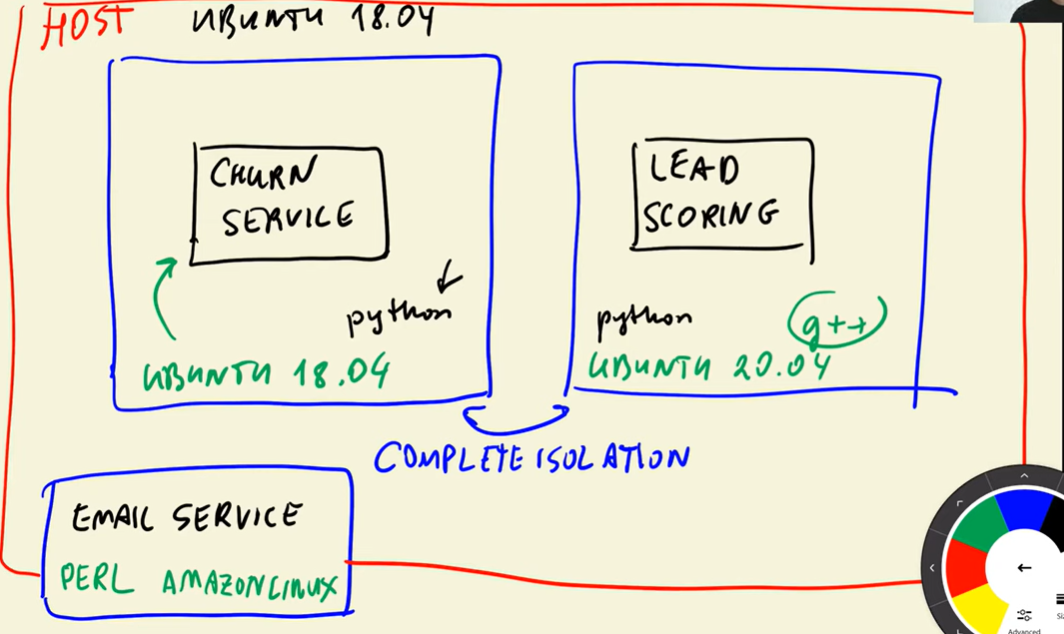
\includegraphics[width=\textwidth]{Images/docker-isolation.png}
	\caption{Docker Isolation}
	\label{fig:11}
\end{figure}
%\FloatBarrier

To get started with Docker for the churn prediction project you can follow the instructions below.

\begin{itemize}
\item On Ubuntu
\begin{lstlisting}[language=python, numbers=none]
sudo apt-get install docker.io
\end{lstlisting}

To run docker without sudo, follow this instruction.

\item On MacOS
	\begin{itemize}[noitemsep, topsep=0pt]
		\item Follow the steps in the \href{https://docs.docker.com/desktop/install/mac-install/}{Docker docs}.
	\end{itemize}
\end{itemize}

To run docker using the default command in python:
\begin{lstlisting}[language=python, numbers=none]
docker run -it --rm python:3.8.12-slim
\end{lstlisting}

We can change the entrypoint to be bash using:
\begin{lstlisting}[language=python, numbers=none]
docker run -it --rm --entrypoint=bash python:3.8.12-slim
\end{lstlisting}

Once our project was packed in a Docker container, we're able to run our project on any machine.  First we have to make a Docker image. In Docker image file, there are settings and dependencies we have in our project. To find Docker images that you need you can simply search the Docker website. 

We can create a Dockerfile where we define everything that we want to do in a docker image. Here is a Dockerfile (There should be no comments in Dockerfile, so remove the comments when you copy)

\begin{lstlisting}[language=python, numbers=none]
# First install the python 3.8, the slim version uses less space
FROM python:3.8.12-slim

# Install pipenv library in Docker 
RUN pip install pipenv

# create a directory in Docker named app and we're using it as work directory 
WORKDIR /app                                                                

# Copy the Pip files into our working derectory 
COPY ["Pipfile", "Pipfile.lock", "./"]

# install the pipenv dependencies for the project and deploy them.
RUN pipenv install --deploy --system

# Copy any python files and the model we had to the working directory of Docker 
COPY ["*.py", "model_C=1.0.bin", "./"]

# We need to expose the 9696 port because we're not able to communicate with Docker outside it
EXPOSE 9696

# If we run the Docker image, we want our churn app to be running
ENTRYPOINT ["gunicorn", "--bind", "0.0.0.0:9696", "predict:app"]
\end{lstlisting}

The flags \smtt{--deploy} and \smtt{--system} makes sure that we install the dependencies directly inside the Docker container without creating an additional virtual environment (which pipenv does by default).

If we don't put the last line ENTRYPOINT, we will be in a python shell. Note that for the entrypoint, we put our commands in double quotes.

After creating the Dockerfile, we need to build it:
\begin{lstlisting}[language=python, numbers=none]
docker build -t churn-prediction .
\end{lstlisting}

To run it, execute the command below:
\begin{lstlisting}[language=python, numbers=none]
docker run -it -p 9696:9696 churn-prediction:latest
\end{lstlisting}

Flag explanations:
\begin{itemize}[noitemsep, topsep=0pt]
\item \smtt{-t}: is used for specifying the tag name ``churn-prediction''.
\item \smtt{-it}: in order for Docker to allow us access to the terminal.
\item \smtt{--rm}: allows us to remove the image from the system after we're done.
\item \smtt{-p}: to map the 9696 port of the Docker to 9696 port of our machine. (first 9696 is the port number of our machine and the last one is Docker container port.)
\item \smtt{--entrypoint=bash}: After running Docker, we will now be able to communicate with the container using bash (as you would normally do with the Terminal). Default is python.
\end{itemize}

At last you've deployed your prediction app inside a Docker continer. 


\section{Online Deployment}
\subsection{Web services: Deploying models with Flask and Docker}
\subsubsection{Creating a Virtual Environment with Pipenv}
To deploy the model, we have to create a virtual environment using \texttt{Pipenv}. In your project folder, create a web-service folder.  This ``web-service'' will house the files required to deploy the application.  We should make sure that the version we used to create the pickle file is the exact same version we install in the virtual environment.
\begin{lstlisting}[language=python, numbers=none]
 pip freeze | grep scikit-learn
\end{lstlisting}

Using the same exact version of scikit-learn, we install that in the virtual environment with ``pipenv''. In the web-service folder, run the command to install the necessary packages using ``pipenv''.
\begin{lstlisting}[language=python, numbers=none]
 pipenv install scikit-learn==1.0.2 flask --python=3.9
\end{lstlisting}

This creates a \texttt{Pipfile} and \texttt{Pipfile.lock} containing the packages we just installed and their exact version. Once the virtual environment have been created, launch the subshell in virtual environment. To enter the virtual environment, run the command below:
\begin{lstlisting}[language=python, numbers=none]
pipenv shell
\end{lstlisting}
The prompt is usually long. We can reduce it using:
\begin{lstlisting}[language=python, numbers=none]
PS1="> "
\end{lstlisting}

\subsubsection{Creating a script for predicting}
To predict, we create a script for prediction called \texttt{predict.py}:

\begin{lstlisting}[language=python, numbers=none]
import pickle

with open('lin_reg.bin', 'rb') as f_in:
    (dv, model) = pickle.load(f_in)

def prepare_features(ride):
    features = {}
    features['PU_DO'] = '%s_%s' % (ride['PULocationID'], ride['DOLocationID'])
    features['trip_distance'] = ride['trip_distance']
    return features

def predict(features):
    X = dv.transform(features)
    preds = model.predict(X)
    return preds[0]
\end{lstlisting}

We can test our prediction with a \texttt{test.py} file
\begin{lstlisting}[language=python, numbers=none]
import predict

ride = {
    "PULocationID": 10,
    "DOLocationID": 50,
    "trip_distance": 40
}

features = predict.prepare_features(ride)
pred = predict.predict(ride)
print(pred)
\end{lstlisting}
To run prediction, we simply run \textbf{\smtt{python test.py}} in terminal.

\subsubsection{Putting the script into a Flask app}
To turn the scripts above to a flask application, we create a function that will be a wrapper around the \texttt{predict.py} and \texttt{test.py} file. This function will take web requests, HTTP request and the score it gets in the request and return the prediction. Let's call the function \texttt{predict\_endpoint()}. Update the \texttt{predict.py} file with the function \texttt{predict\_endpoint()}.

\begin{lstlisting}[language=python, numbers=none]
import pickle
from flask import Flask, request, jsonify

with open('lin_reg.bin', 'rb') as f_in:
    (dv, model) = pickle.load(f_in)

def prepare_features(ride):
    features = {}
    features['PU_DO'] = '%s_%s' % (ride['PULocationID'], ride['DOLocationID'])
    features['trip_distance'] = ride['trip_distance']
    return features

def predict(features):
    X = dv.transform(features)
    preds = model.predict(X)
    return float(preds[0])
  
app = Flask('duration-prediction')

@app.route('/predict', methods=['POST']) # turn predict function into an endpoint
def predict_endpoint():
    ride = request.get_json()

    features = prepare_features(ride)
    pred = predict(features)

    result = {
        'duration': pred
    }
    return jsonify(result)


if __name__ == "__main__":
    app.run(debug=True, host='0.0.0.0', port=9696)
\end{lstlisting}
In the above code, we added an import for Flask, requests and jsonify. Requests gives us a way get the data,  the result of our prediction will be a dictionary with duration and jsonify returns this as a \texttt{json} object. We also added a decorator which adds some extra functionality to the predict function by turning the function into HTTP endpoint and we can start sending requests to this endpoint and get responses.  This library has a method called ``POST'' that we use for sending post requests and here we need to specify the url end point and port to which we want to send the request.

We update the \texttt{test.py} file with the \textbf{\smtt{url}} variable and \textbf{\smtt{response}} variable.
\begin{lstlisting}[language=python, numbers=none]
import requests
import predict

ride = {
    "PULocationID": 10,
    "DOLocationID": 50,
    "trip_distance": 40
}

url = 'http://localhost:9696/predict'
response = requests.post(url, json=ride)
print(response.json())
\end{lstlisting}

The \texttt{requests} library is used for making HTTP requests in Python. The \textbf{\smtt{url}} variable contains the address of the local server endpoint \textbf{\smtt{/predict}} running on port 9696. The \textbf{\smtt{requests.post}} method is used to send a POST request to the \textbf{\smtt{url.}} The \textbf{\smtt{json}} parameter is used to send the \textbf{\smtt{ride}} dictionary as a JSON payload in the request body. The response from the server is stored in the \textbf{\smtt{response}} variable. The \textbf{\smtt{response.json()}} method is called to parse the JSON response from the server into a Python dictionary. The parsed response is then printed to the console.

The code in the \texttt{test.py} file sends a POST request to a local server to get a prediction based on the provided ride details. In the prompt in the virtual environment, we run \textbf{\texttt{python predict.py}} and open another terminal to run \textbf{\texttt{python test.py}}.  Now we have sucessfully put our model in a flask and deployed that model in a development environment. Alternatively, we can install gunicorn if we want to put this into production. The application we just ran is running in a development environment in Flask. To run it in a production environment, we use gunicorn.  We first install gunicorn

\begin{lstlisting}[language=python, numbers=none]
pipenv install gunicorn
\end{lstlisting}

Then start the service using:
\begin{lstlisting}[language=python, numbers=none]
gunicorn --bind 0.0.0.0:9696 predict:app 
\end{lstlisting}
Then test the the service and make prediction with \textbf{\texttt{python test.py}}.

\subsubsection{Packaging the app to Docker}
To package the app to \texttt{Docker}, first we need to create a ``Dockerfile''. In the Dockerfile, we add the following command:
\begin{lstlisting}[language=python, numbers=none]
FROM python:3.9.18-slim

RUN pip install -U pip
RUN pip install pipenv

WORKDIR /app  

COPY ["Pipfile", "Pipfile.lock", "./"]

RUN pipenv install --deploy --system

COPY ["predict.py", "lin_reg.bin", "./"]

EXPOSE 9696

ENTRYPOINT ["gunicorn", "--bind=0.0.0.0:9696", "predict:app"]
\end{lstlisting}

Next we build the docker image using the Dockerfile
\begin{lstlisting}[language=python, numbers=none]
docker build -t ride-duration-prediction-service:v1 .
\end{lstlisting}

And then we can test it in interactive mode (``--it'') and remove it after running (``-p'') using:
\begin{lstlisting}[language=python, numbers=none]
docker run -it --rm -p 9696:9696 ride-duration-prediction-service:v1 
\end{lstlisting}

In a separate shell, test the the service and make prediction with \textbf{\texttt{python test.py}}. With the docker container, we can serve our model and deploy the service anywhere docker is supported .e.g., using AWS Elastic Beanstalk or Kubernetes.

\subsection{Web services: Getting the models from the model registry (MLflow)} --- Not up to date
\begin{enumerate}
    \item \textbf{Overview:}
    \begin{itemize}
        \item Discussed combining model deployment using Flask with model registry.
        \item Deployed a linear regression model as a web service.
        \item Exposed predictive function as an endpoint for making predictions.
    \end{itemize}
    
    \item \textbf{Model Registry Integration:}
    \begin{itemize}
        \item Utilized model registry to fetch models (e.g., random forest) using a run ID.
        \item Demonstrated setting up MLflow server with SQLite and S3 as the artifact root.
    \end{itemize}
    
    \item \textbf{Implementation Steps:}
    \begin{itemize}
        \item Prepared functions for data conversion and prediction.
        \item Created Flask application to deploy model fetched from MLflow registry.
        \item Demonstrated setting up virtual environment and installing dependencies.
    \end{itemize}
    
    \item \textbf{Simplifying Model Handling:}
    \begin{itemize}
        \item Emphasized using scikit-learn pipelines to combine preprocessing and model into a single entity.
        \item Demonstrated logging entire pipeline to MLflow, reducing complexity in fetching artifacts.
    \end{itemize}
    
    \item \textbf{Testing and Validation:}
    \begin{itemize}
        \item Validated the new pipeline-based model by running predictions and comparing outputs.
        \item Highlighted the importance of specifying model version in responses.
    \end{itemize}
    
    \item \textbf{Independence from Tracking Server:}
    \begin{itemize}
        \item Addressed potential issues with dependency on tracking servers.
        \item Demonstrated fetching models directly from S3 to avoid dependency on MLflow tracking server.
        \item Suggested using environment variables for dynamic configuration in deployments (e.g., Kubernetes).
    \end{itemize}
    
    \item \textbf{Code and Configuration:}
    \begin{itemize}
        \item Provided code snippets for setting up and testing Flask application.
        \item Showed how to replace hardcoded paths with environment variables for flexible deployment.
    \end{itemize}
\end{enumerate}

\subsubsection*{Example Code Snippets:}
\textbf{Creating a Pipeline:}
\begin{verbatim}
from sklearn.pipeline import make_pipeline

pipeline = make_pipeline(vectorizer, RandomForestRegressor())
pipeline.fit(X_train, y_train)
\end{verbatim}

\textbf{Logging Pipeline to MLflow:}
\begin{verbatim}
mlflow.sklearn.log_model(pipeline, "model")
\end{verbatim}

\textbf{Fetching Model from S3:}
\begin{verbatim}
model_uri = f"s3://my-bucket/mlflow/{run_id}/artifacts/model"
model = mlflow.sklearn.load_model(model_uri)
\end{verbatim}

\textbf{Using Environment Variables:}
\begin{verbatim}
import os

run_id = os.getenv('RUN_ID')
model_uri = f"s3://my-bucket/mlflow/{run_id}/artifacts/model"
model = mlflow.sklearn.load_model(model_uri)
\end{verbatim}


\subsection{Batch: Preparing a scoring script}
Assuming we have built a model to predict the ride duration and we want to see how our drivers deviate from the actual duration, we can deploy the model for predicting ride duration in batch mode. In deploying our model using Batch deployment, we have to train the model in a notebook, apply the model and then turn the notebook into a script.

To convert our \smtt{score.ipynb} notebook to a script, use: 
\begin{lstlisting}[language=python, numbers=none]
jupyter nbconvert --to script score.ipynb
\end{lstlisting}

After turning the notebook into a script, we have to clean the script, parametrize the script and make it self-contained in such a way that we can just run the script and get the predictions.  After this step, the next step is to deploy the model or schedule the script with Prefect.

Once the script is ready, we can create an environment with pipenv and specify all the dependencies that the script has. We also want to save the result to S3 in this case, we would need credentials to do that.  after that, you package the script in a docker container and schedule your docker container with AWS Batch or ECS or as a kubernetes job.


%--------------- Chapter 5: Monitoring -----------%
\chapter{Model Monitoring} \label{ch:5}
\inspiration{Model monitoring is the ongoing process of tracking, analyzing, and evaluating the performance and behavior of machine learning models in real-world, production environments. It involves measuring various data and model metrics to help detect issues and anomalies and ensure that models remain accurate, reliable, and effective over time.}{\href{https://www.evidentlyai.com/ml-in-production/model-monitoring}{EvidentlyAI Blog}}{}

\section{Introduction to ML monitoring}

 \begin{funfact}[frametitle=\facttitlep{Fun Fact}{Challenges in ML Model Deployment}]
Implementing a machine learning model is challenging, but building production services with that model is even harder. Over time, a model's performance may degrade, necessitating monitoring to maintain quality.
\end{funfact}

Once we've built a machine learning model, after sometime, the model's performance starts to degrade.  ML model monitoring involves tracking a predefined set of metrics to detech issues and answer questions like ``What happened?'' and ``Is the system working as expected?'' This module discusses how to monitor machine learning models in production, focusing on maintaining model performance over time. Machine learning monitoring is done to monitor:
\begin{itemize}[noitemsep, topsep=0pt]
\item Service Health
	\begin{itemize}
		\item Latency
		\item Memory
		\item Uptime
	\end{itemize}
\item Data Health
	\begin{itemize}
		\item Data Drift
		\item Broken Pipelines
		\item Data Outage
		\item Schema Change
		\item Underperforming Segments
	\end{itemize}
\item Model Health
	\begin{itemize}
		\item Model Accuracy
		\item Concept Drift
		\item Model Bias
	\end{itemize}
\end{itemize}

\texttt{\textbf{Service Health Monitoring}} - Service health monitoring is essential to ensure the service operates correctly. Key metrics include uptime, memory usage, and latency.

\texttt{\textbf{Model Performance Metrics}} - Additional Layers for ML Models: Include metrics related to data and model performance. Model performance metrics monitors model performance and is dependent on the problem statement. For ranking algorithms, use ranking metrics; for regression problems, use metrics like mean absolute error (MAE) or mean absolute percentage error (MAPE). For classification problems, use metrics like log loss, precision, and recall.

\texttt{\textbf{Data Quality and Integrity Metrics}} -  In cases where ground truth is delayed, use proxy metrics related to data quality and integrity.  Monitor metrics like the share of missing values, value ranges, and data distribution changes.

\texttt{\textbf{Data Drift and Concept Drift}} -  Monitor data drift and concept drift to detect changes in data distributions over time. We compare input data distributions and model outputs over time to detect drifts.These metrics serve as early signals of potential problems with the model.

\texttt{\textbf{Extended Metrics for Monitoring}}
\begin{itemize}[noitemsep, topsep=0pt]
    \item Depending on the sensitivity of your case and risks, consider additional metrics such as:
    \begin{itemize}
        \item Quality metrics by segments (e.g., category-specific performance).
        \item Model bias and fairness, especially in sensitive domains like healthcare or finance.
        \item Outlier monitoring to reduce risks by sending specific objects to manual review.
        \item User trust metrics for recommender systems, especially for explaining recommendations.
    \end{itemize}
\end{itemize}

\newpage
\subsection{Batch and Online Model Monitoring}

    \begin{mathaside}[frametitle=\mathtitle{Importance \color{firebrick}{of Monitoring}}]
       Monitoring  \texttt{production services} is crucial to ensure they function correctly. For machine learning models, additional layers of monitoring related to data and model performance are required. Important aspects to monitor include model performance, data drift, and concept drift.
    \end{mathaside}

\texttt{\textbf{Batch Monitoring}}
\begin{itemize}[noitemsep, topsep=0pt]
    \item Involves running evaluation jobs periodically or based on triggers.
    \item Daily monitoring jobs query model prediction logs to compute model and data quality metrics.
    \item Suitable for batch data pipelines and online ML services.
    \item Easier to maintain than continuous monitoring services.
    \item Combines immediate and delayed monitoring within the same architecture.
    \item Can run data validation jobs alongside monitoring.
    \item Introduces delays in metric computation.
    \item Requires expertise in workflow orchestration and data engineering resources.
\end{itemize}

\texttt{\textbf{Real-Time Monitoring}}
\begin{itemize}[noitemsep, topsep=0pt]
    \item Data is sent directly from the ML service to the monitoring service.
    \item Continuously computes and publishes ML quality metrics.
    \item Suitable for online ML prediction services.
    \item Allows near real-time detection of issues like missing data.
    \item More costly in terms of engineering resources.
    \item Batch monitoring pipelines may still be needed for delayed ground truth.
\end{itemize}

Use existing monitoring tools and dashboards (like Grafana) to monitor ML models.  For batch models, metrics like data drift and precision can be calculated on batches of data. For online models, use window functions to generate small batches for calculating metrics.

\subsection{Monitoring Architecture}
\begin{itemize}[noitemsep, topsep=0pt]
    \item We can build a general monitoring scheme applicable to both batch and non-batch models.
    \item Start with prediction logs from the service (batch or online).
    \item Create a monitoring pipeline that reads prediction logs, calculates metrics, and stores them in a database.
    \item Use a dashboard tool like Grafana to visualize and monitor these metrics.
\end{itemize}

\begin{figure}[h]
	\centering
	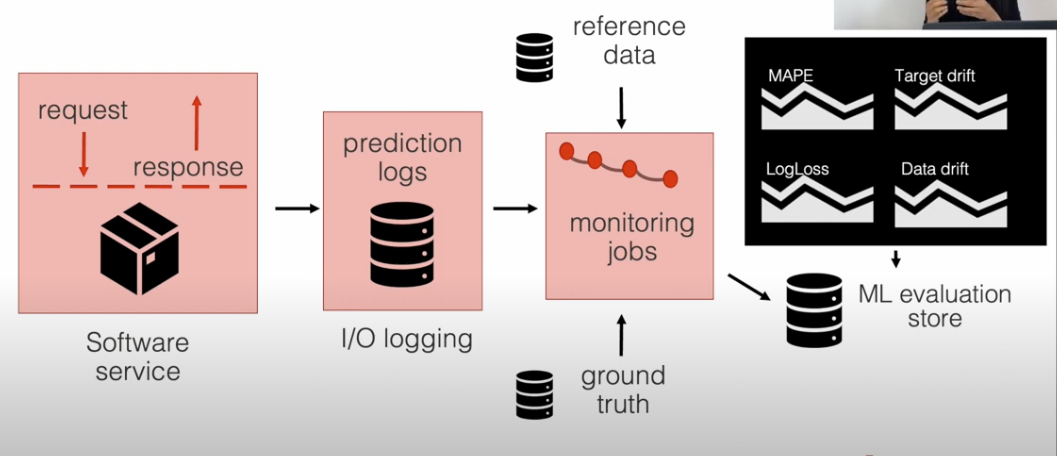
\includegraphics[width=\textwidth]{Images/monitoring-scheme.png}
	\caption{Monitoring Scheme}
	\label{fig:12}
\end{figure}
%\FloatBarrier

\subsection{Practical Implementation}
For batch models, use BI tools like Tableau or Looker for initial analysis. For online models, simulate production usage and build monitoring on top of logs using tools like Prefect and Evidently. Store metrics in a PostgreSQL database and visualize them using Grafana.
\begin{itemize}
    \item Logging and Monitoring Pipeline:
    \begin{itemize}
        \item Prediction Logs: Collect logs from the service.
        \item Batch Analysis: Analyze logs in batches to calculate metrics.
        \item Database Storage: Store metrics in a database.
        \item Dashboarding: Use tools like Grafana to visualize and monitor metrics.
    \end{itemize}
    \item Tools Used:
    \begin{itemize}
        \item Prefect: For scheduling and running monitoring jobs.
        \item Evidently Library: For calculating and comparing metrics.
        \item PostgreSQL: For storing calculated metrics.
        \item Grafana: For creating dashboards and alerts.
    \end{itemize}
\end{itemize}

\section{ML Monitoring Environment Setup}
To setup environment for monitoring for our project, in the project folder,
\begin{lstlisting}[language=python, numbers=none]
 mkdir taxi-monitoring
\end{lstlisting}
Change directory into the ``taxi-monitoring'' folder and create a virtual environment.
\begin{lstlisting}[language=python, numbers=none]
conda create -n monitoring-env python=3.11
\end{lstlisting}

Next we activate the virtual environment
\begin{lstlisting}[language=python, numbers=none]
conda activate monitoring-env 
\end{lstlisting}

Create a \smtt{requirements.txt} file to list all the packages and install it. Once the requirements have been listed in the requirement file, install it in the terminal with:
\begin{lstlisting}[language=python, numbers=none]
pip install -r requirements.txt
\end{lstlisting}

Next we create a docker compose file. Docker compose is a tool that allows us to build multi-container docker application.  Docker compose ``yaml'' file is a file where you can list all your services.  The docker compose file is created below.
\begin{lstlisting}[language=python, numbers=none]
version: '3.7'

volumes: 
	grafana_data: {}

networks:
	front-tier:
	back-tier:
	.....

\end{lstlisting}

In the ``taxi-monitoring'' directory, create a ``config'' folder and a ``grafana\_datasources.yaml'' file. Docker compose is going to allow us to create all the services. Run the docker compose build command using:
\begin{lstlisting}[language=python, numbers=none]
docker-compose up --build
\end{lstlisting}

If you get the error below when building the docker file,  find and kill the process using the port. 

\begin{lstlisting}[language=python, numbers=none]
Error response from daemon: Ports are not available: exposing port TCP 0.0.0.0:5432 -> 0.0.0.0:0: listen tcp 0.0.0.0:5432: bind: address already in use
\end{lstlisting}

Run the following one after the other
\begin{lstlisting}[language=python, numbers=none]
sudo lsof -i :5432
sudo kill -9 <PID>
\end{lstlisting}

Once docker compose is up and running, we can try to access grafana using \smtt{localhost:3000/login}, default username and password is \smtt{admin}.  We can access adminer at \smtt{http://localhost:8080/}. We have successfully created our working environment and made sure our services starts. Once the service starts, we can prepare reference data and model. 

\section{Evidently Metric Calculation}
To perform metric calculation in Evidently, we need to create a report. A report is an object which allows us to select what metrics we want to calculate and group them all together. The code snippet provided defines a \texttt{Report} object with specific metrics to evaluate in a dataset. Below is a detailed breakdown of what each part does:

\subsection*{Code Snippet}
\begin{lstlisting}[language=python, numbers=none]
report = Report(metrics=[
    ColumnDriftMetric(column_name='prediction'),
    DatasetDriftMetric(),
    DatasetMissingValuesMetric()
])
\end{lstlisting}

\subsection*{Explanation}
\begin{itemize}
    \item \texttt{report = Report(metrics=[...])}: This initializes a \texttt{Report} object with a list of metrics that will be calculated when the report is generated.
    
    \item \texttt{ColumnDriftMetric(column\_name='prediction')}: This metric checks for drift in the specified column, which is \texttt{'prediction'} in this case. Drift indicates that the statistical properties of a column have changed over time, which can signal issues such as changes in the underlying data distribution or model degradation.
    
    \item \texttt{DatasetDriftMetric()}: This metric evaluates the entire dataset to detect drift. It assesses if the overall data distribution has changed, which can affect the performance and reliability of models trained on the dataset.
    
    \item \texttt{DatasetMissingValuesMetric()}: This metric checks for missing values in the dataset. It identifies the presence and possibly the extent of missing data, which is crucial for maintaining data quality and ensuring the accuracy of analysis and model training.
\end{itemize}

\subsection*{Example Usage}
This setup is typically used in monitoring data quality and model performance over time. Here is how you might use it:

\subsection*{1. Initialize the Report}
\begin{lstlisting}[language=python, numbers=none]
report = Report(metrics=[
    ColumnDriftMetric(column_name='prediction'),
    DatasetDriftMetric(),
    DatasetMissingValuesMetric()
])
\end{lstlisting}

\subsection*{2. Generate the Report with Data}
Assuming you have current and reference datasets (for drift comparison):
\begin{lstlisting}[language=python, numbers=none]
current_data = ...  # Load or define your current dataset
reference_data = ...  # Load or define your reference dataset

report.run(current_data=current_data, reference_data=reference_data)
\end{lstlisting}

\subsection*{3. View the Report}
After running the report, you can inspect the results:
\begin{lstlisting}[language=python, numbers=none]
print(report.show())
\end{lstlisting}

\subsection*{Practical Application}
In a real-world scenario, you would use this type of report to continuously monitor your data pipeline. For instance:
\begin{itemize}
    \item \textbf{Column Drift Monitoring}: Ensuring that your model predictions remain consistent over time and are not being affected by unforeseen changes in data distribution.
    \item \textbf{Dataset Drift Monitoring}: Detecting shifts in your overall data, which could indicate changes in user behavior, data collection issues, or other external factors.
    \item \textbf{Missing Values Monitoring}: Keeping track of missing data to maintain data integrity and avoid biases in your analysis or model training.
\end{itemize}

We can create the report object as a python dictionary. This allows us to derive any value for the dictionary.We could derive information such as the prediction drift,  number of drifted columns, and about the shares of missing value. By regularly generating and reviewing such reports, you can proactively address data quality issues and maintain the performance and reliability of your data-driven applications.

\section{Evidently Monitoring Dashboard}
An example of the Evidently monitoring dashboard can be found \href{https://github.com/chuksoo/mlops-zoomcamp-2024/blob/main/05%20-%20Monitoring/taxi-monitoring/baseline_model_nyc_taxi_data.ipynb}{here}. Once the dashboard have been created in jupyter notebook, we can test iot in the terminal by calling Evidently UI.  In the ``taxi-monitoring'' directory, run \smtt{evidently ui} which starts the monitoring service. You can copy the URL, and paste in the browser to see the project list.  We notice that we don't have any visible dashboard. In this case, we have to configure it using the code snippet below:

\begin{lstlisting}[language=python, numbers=none]
# configure the dashboard
project.dashboard.add_panel(
    DashboardPanelCounter(
        filter=ReportFilter(metadata_values={}, tag_values=[]),
        agg=CounterAgg.NONE,
        title="NYC taxi data dashboard"
    )
)

project.dashboard.add_panel(
    DashboardPanelPlot(
        filter=ReportFilter(metadata_values={}, tag_values=[]),
        title="Inference Count",
        values=[
            PanelValue(
                metric_id="DatasetSummaryMetric",
                field_path="current.number_of_rows",
                legend="count"
            ),
        ],
        plot_type=PlotType.BAR,
        size=WidgetSize.HALF,
    ),
)

project.dashboard.add_panel(
    DashboardPanelPlot(
        filter=ReportFilter(metadata_values={}, tag_values=[]),
        title="Number of Missing Values",
        values=[
            PanelValue(
                metric_id="DatasetSummaryMetric",
                field_path="current.number_of_missing_values",
                legend="count"
            ),
        ],
        plot_type=PlotType.LINE,
        size=WidgetSize.HALF,
    ),
)

project.save()
\end{lstlisting}

Once we've completed the configuration, we save and run it. We can go back to the monitoring service URL to see the dashboard.  Our dashboard looks like the figure below.
\begin{figure}[h]
	\centering
	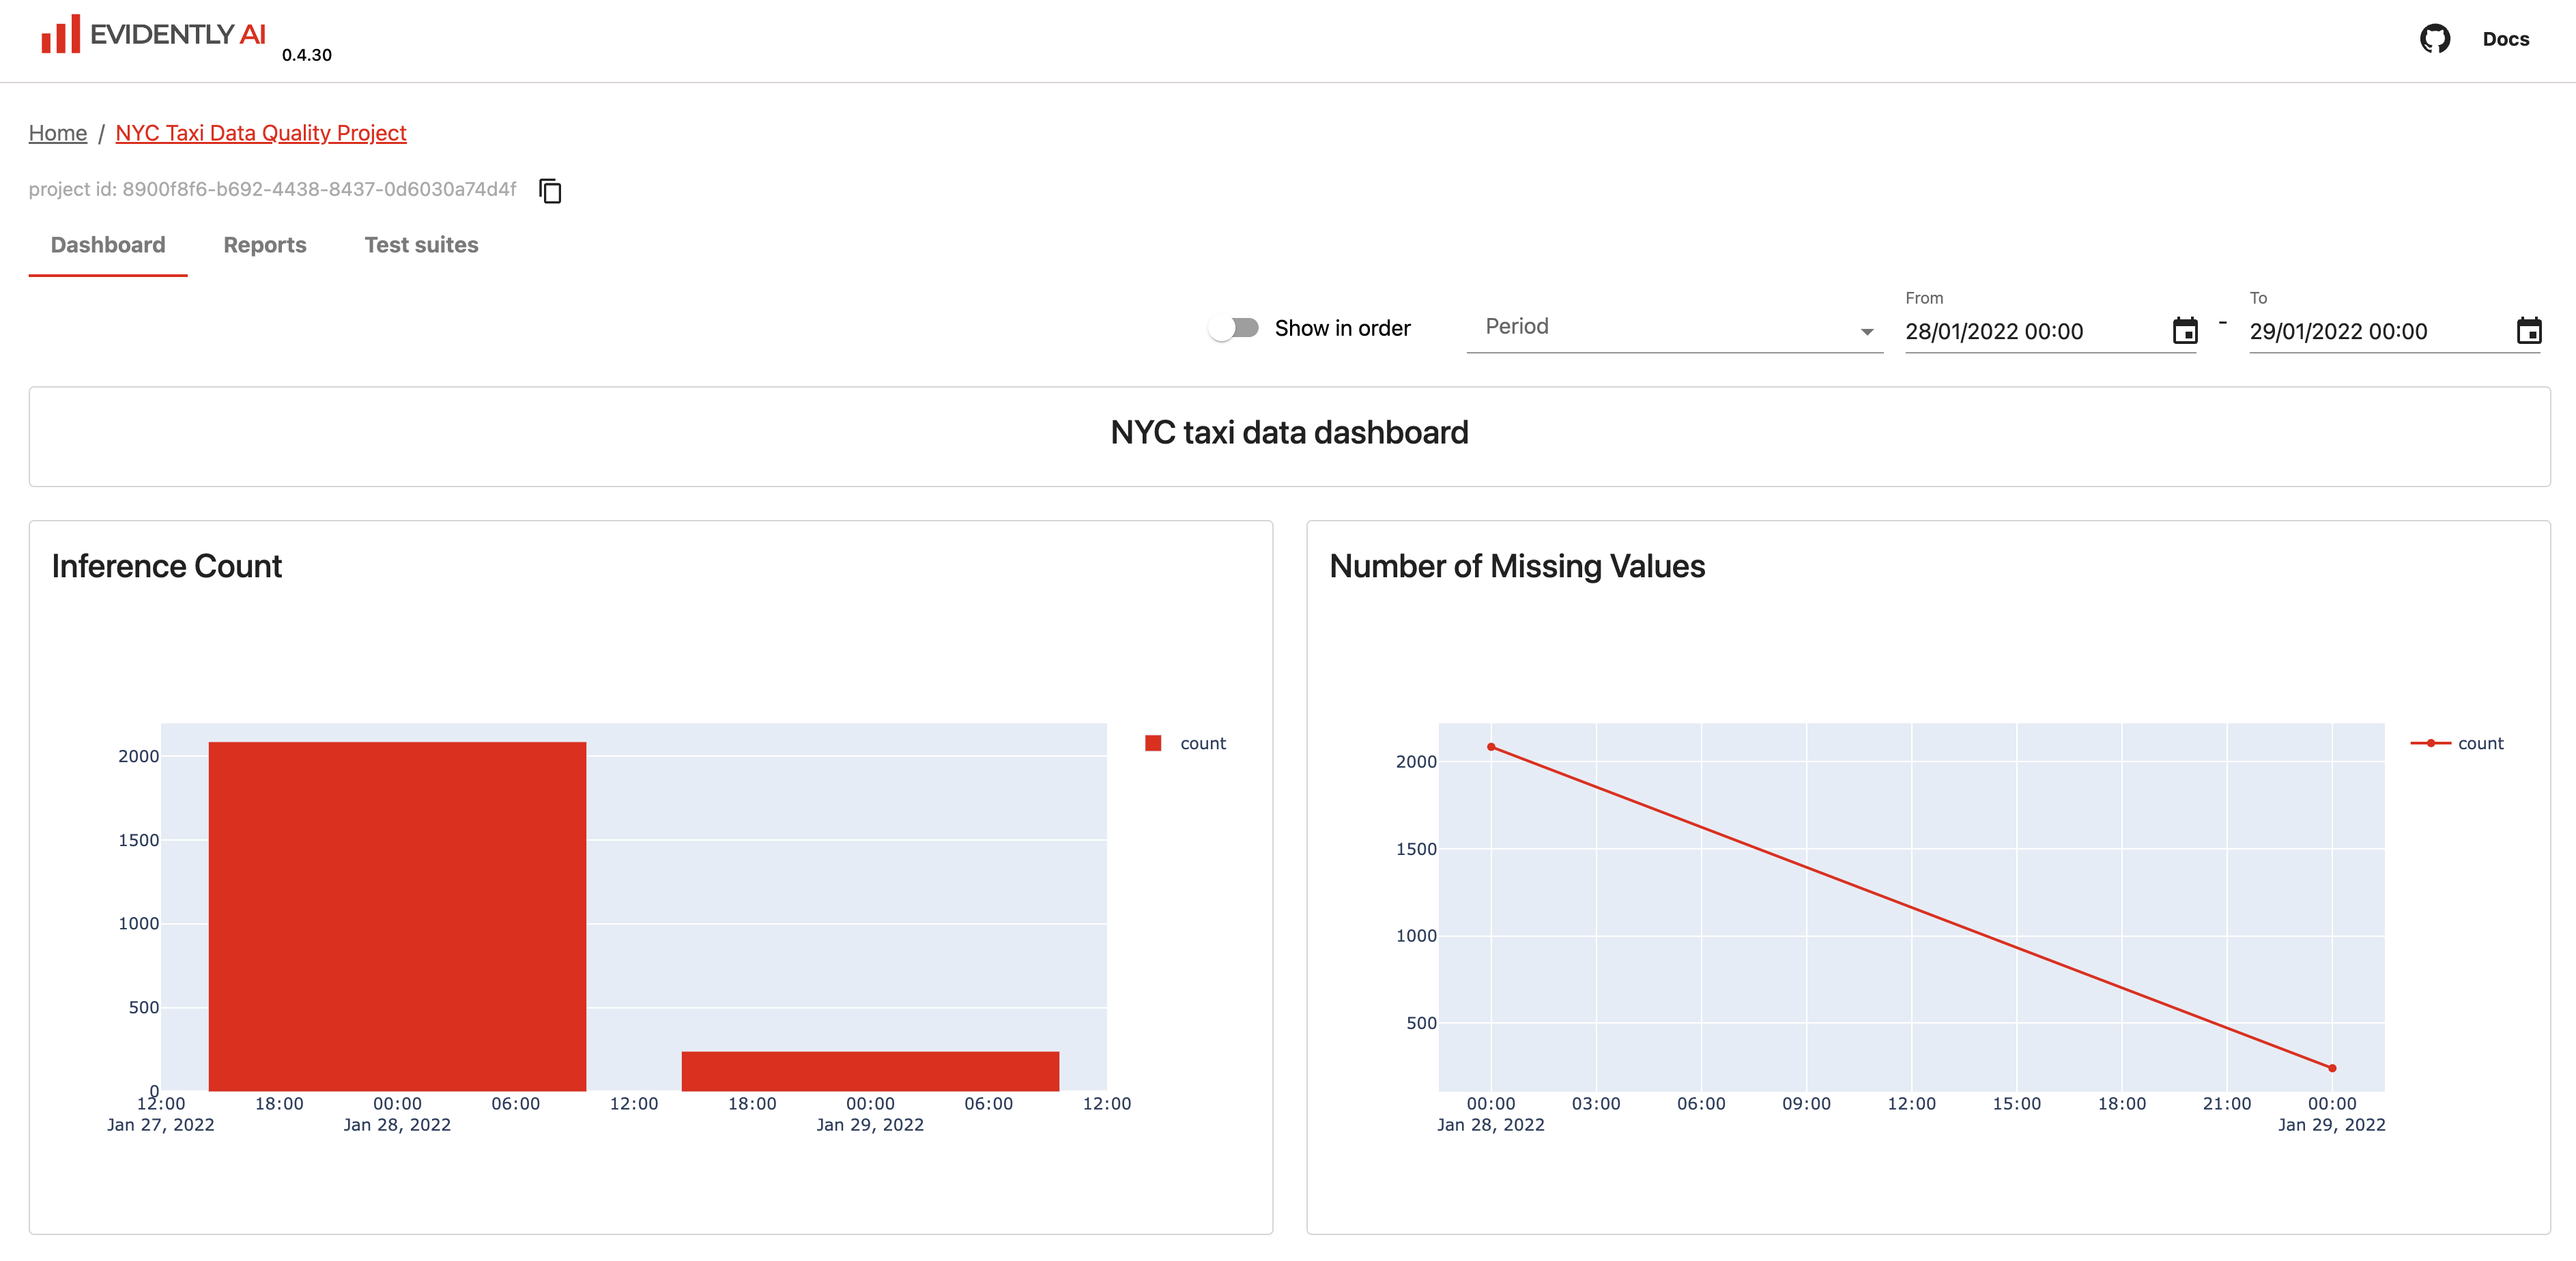
\includegraphics[width=\textwidth]{Images/evidently-dashboard.png}
	\caption{Evidently Monitoring Dashboard}
	\label{fig:13}
\end{figure}
\FloatBarrier
With the dashboard, we can build pretty nice reports to monitor your data and models especially for batch models deployed in production very quickly.

\section{Data Quality Monitoring}
Here we describes ways to modify a script to create a data monitoring dashboard. 
\subsubsection{Load Reference Data and Model}
\begin{itemize}[noitemsep, topsep=0pt]
\item Script now includes functions to load reference data and a model.
\end{itemize}
\subsubsection{Daily Data Processing}
\begin{itemize}[noitemsep, topsep=0pt]
\item We read all data initially.
\item Simulates daily usage by processing data in 10-second intervals.
\item Creates a current data set for each simulated day.
\end{itemize}
\subsubsection{Report Generation}
\begin{itemize}[noitemsep, topsep=0pt]
\item Existing report generation code is reused to transform data.
\item Script calculates metrics like prediction drift, drifted columns, and missing value share.
\end{itemize}
\subsubsection{Database Update}
\begin{itemize}[noitemsep, topsep=0pt]
\item We then insert calculated metrics into a database table.
\end{itemize}
We can also convert the script into a Prefect pipeline using decorators. In data quality monitoring, we used Grafana to visualize the metrics. We populate the dashboard with data for prediction drift, number of drifted columns, and missing value share.

\section{Saving and Reusing Grafana Dashboards}
In order to save and reuse Grafana dashboards, first we create a configuration file, update docker compose, and configure the dashboard.

\textbf{Steps:}
\begin{enumerate}
\item \textbf{Configuration Files:}
	\begin{itemize}[noitemsep, topsep=0pt]
   	\item Create a YAML file (\smtt{grafana\_dashboards.yaml}) in the \textbf{\smtt{config}} directory to specify general dashboard settings.
   	\item Create a directory named \textbf{\smtt{dashboard}} to store individual dashboard configurations.
     	\item Inside \textbf{\smtt{dashboard}}, create a JSON file (e.g., \smtt{data\_drift.json}) for each specific dashboard. This file will store detailed configurations for that dashboard.
	\end{itemize}
\item \textbf{Update Docker Compose:}
	\begin{itemize}[noitemsep, topsep=0pt]
   	\item Modify the \texttt{volumes} section of your Grafana service in \smtt{docker-compose.yml}.
   	\item Add volume mounts for the \smtt{grafana\_dashboards.yaml} file and the \textbf{\smtt{dashboard}} directory. This allows Grafana to access the configuration files during startup.
\begin{lstlisting}[language=python, numbers=none]
    volumes:
      - ./config/grafana_dashboards.yaml:/etc/grafana/provisioning/dashboards/dashboards.yaml:ro
      - ./dashboards:/opt/grafana/dashboards
\end{lstlisting}
	\end{itemize}
\item \textbf{Configure Dashboard JSON:}
	\begin{itemize}[noitemsep, topsep=0pt]
   	\item In Grafana, access the settings for your desired dashboard.
   	\item Export the dashboard configuration as a JSON model.
   	\item Paste the exported JSON code into the corresponding JSON file (e.g., \smtt{data\_drift.json}) within the \textbf{\smtt{dashboard}} directory.
	\end{itemize}
\end{enumerate}

Once, we've edited the code, we then build docker-compose. In the terminal, run \smtt{docker-compose up --build}. In a second terminal,  run \smtt{python evidently\_metrics\_calculation.py}. Once docker is up and running, check the dashboard by login into Grafana at \smtt{http://localhost:3000}. We should see a dashboard like \textbf{Fig. \ref{fig:15}}.
\begin{figure}[h]
	\centering
	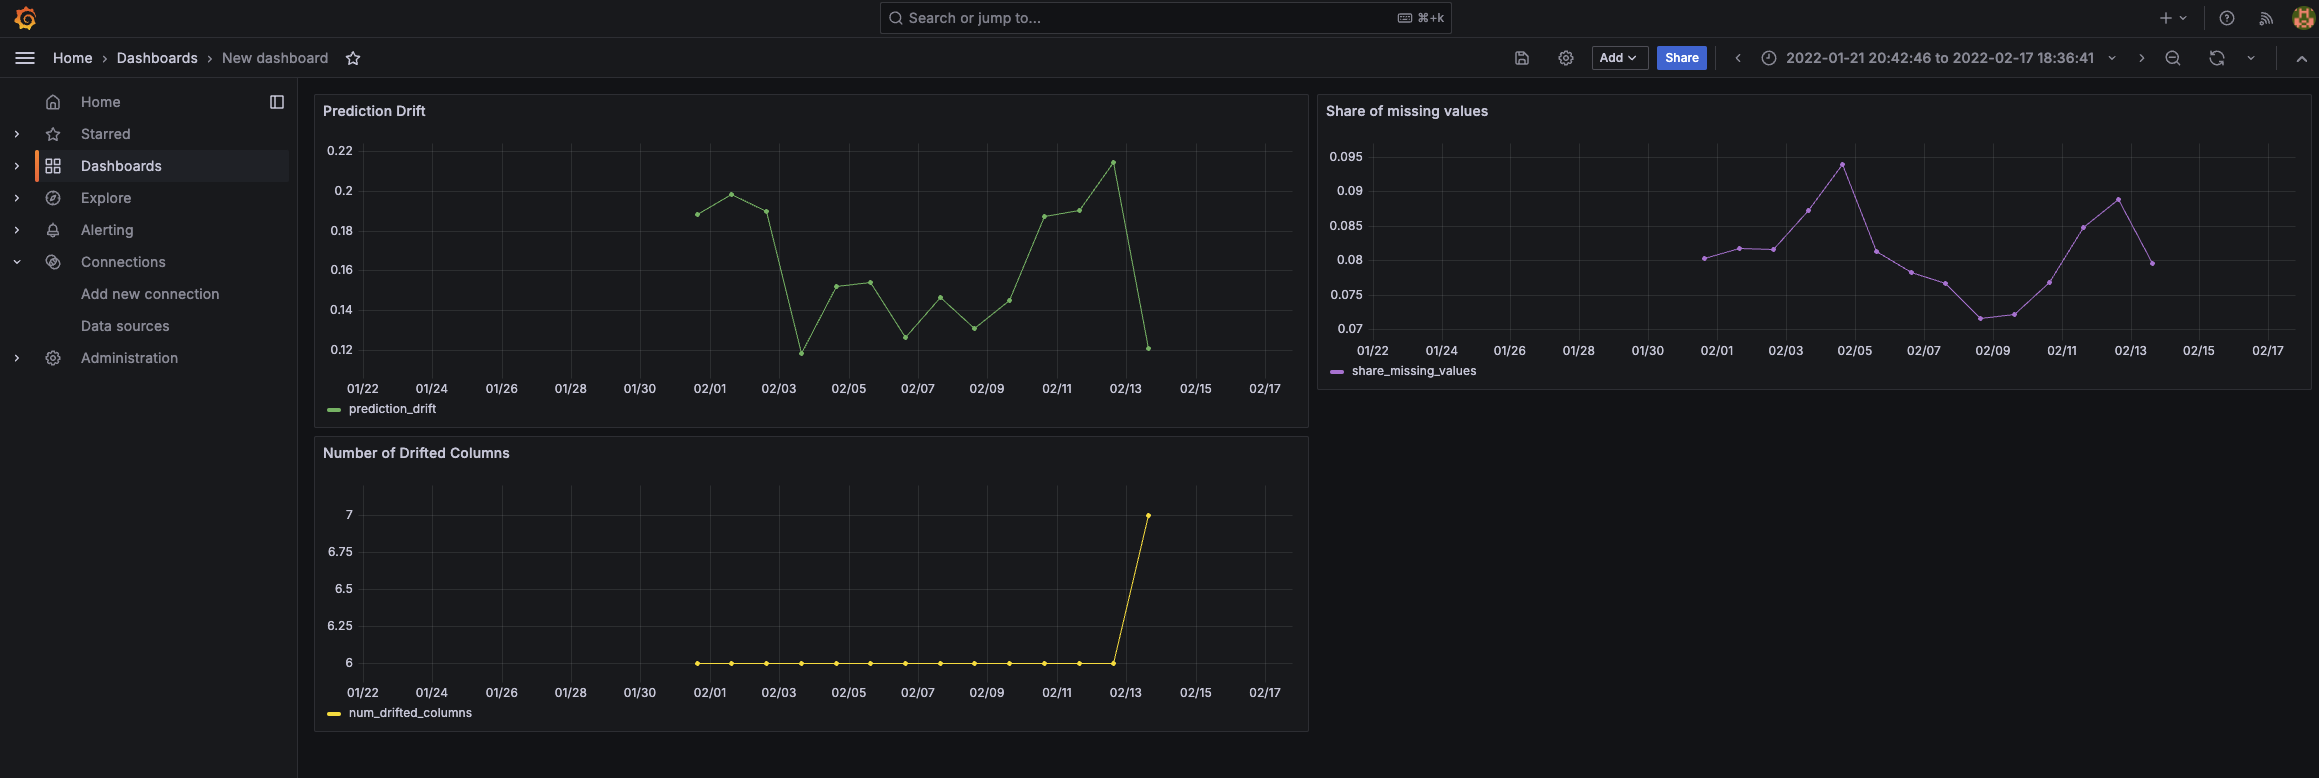
\includegraphics[width=\textwidth]{Images/grafana-dashboard.png}
	\caption{Grafana Saved Dashboard}
	\label{fig:15}
\end{figure}
\FloatBarrier

\section{Debugging with Evidently Library}
This document outlines the debugging process using Evidently library for data and model issues identified through monitoring.

\subsection{Benefits of Evidently}

Evidently offers various functionalities for data monitoring and debugging:

\begin{enumerate}
  \item \textbf{Visual Reports:} Generate visual dashboards to understand data drift and other issues.
  \item \textbf{Test Suites:} Provide pre-defined tests to check for specific data or model problems.
  \item \textbf{Detailed Analysis:} Offer in-depth analysis of data changes and potential causes.
\end{enumerate}

\subsection{Using Evidently for Debugging}

The following steps demonstrate how to use Evidently for debugging:

\begin{enumerate}
  \item \textbf{Import Libraries:} Import necessary libraries like ``evidently'' for reports and test suites, specific metric libraries, and test preset libraries.

  \item \textbf{Load Data:} Load separate reference data (used for training) and current data.

  \item \textbf{Load Model:} Load the model you intend to debug.

  \item \textbf{Prepare Data:} Select the problematic part of the current data for analysis.

  \item \textbf{Using Test Suites:}
    \begin{itemize}[noitemsep, topsep=0pt]
      \item Define ``column\_mappin'' to specify feature mapping between reference and current data.
      \item Exclude target columns if not relevant (e.g., ``Target=None'').
      \item Use \smtt{evidently.test\_presets.DataDriftPreset} for data drift tests.
      \item Run the test suite with \smtt{suite.run(reference\_data, current\_data, column\_mapping)}.
      \item Visualize results using \smtt{suite.show(inline=True)}.
    \end{itemize}

  \item \textbf{Using Reports:}
    \begin{itemize}[noitemsep, topsep=0pt]
      \item Create a report object using ``evidently.Report'' and specify metrics (e.g., \smtt{evidently.Report(evidently.MetricPreset.DATA\_DRIFT)}).
      \item Run the report with \smtt{report.run(reference\_data, current\_data, column\_mapping)}.
      \item Visualize results using ``report.show(inline=True)'' or save as HTML for offline viewing (\smtt{report.save\_html(``report.html'')}).
    \end{itemize}
\end{enumerate}

Evidently's test suites and reports provide valuable tools for debugging data and model issues. They offer clear visualizations and detailed analysis to identify and address data drift and other performance problems.

%--------------- Chapter 6: Best Practices -----------%
\chapter{Best Practices} \label{ch:6}

\section{Testing Python Code with pytest}
In this section, we covers adding unit tests to a Lambda function that processes a stream of events, extracts features, and makes predictions. To perform unit test, we need to set up the testing environment. 
\subsection*{Setting Up the Environment}
To test python code with pytest, first the code for the Lambda function is placed in a separate folder named ``code''. A new folder named ``tests'' is created to store the unit tests. To setup the environment,  python environment is set up using ``pipenv''. This installs dependencies from the ``Pipfile.lock'' file.
\begin{lstlisting}[language=python, numbers=none]
pipenv install
\end{lstlisting}

The pytest library is installed for writing tests. We can install that using:
\begin{lstlisting}[language=python, numbers=none]
pipenv install --dev pytest
\end{lstlisting}

We need to configure VS Code to recognize the Python environment so we can run test from it.  To select the right python interpreter for our test to run locally, we can run:
\begin{lstlisting}[language=python, numbers=none]
pipenv --venv
\end{lstlisting}
This would output something like:
\begin{lstlisting}[language=python, numbers=none]
/Users/chuksokoli/.local/share/virtualenvs/code-dGaX0KrP
\end{lstlisting}
We can now select this environment using \smtt{SHIFT + CTRL + P} for local testing. To ensure ``pytest'' runs in the virtual environment, run \smtt{pipenv shell}. Confirm we are testing in the virtual environment by running \smtt{which pytest}. 

\subsection*{Configuring Python Tests}
We can configure through the ``Testing'' icon in VSCode. You have to be on the ``code'' directory. We select a testing framework to enable and chose the ``tests'' folder as the directory containing the tests. We create a docker file and build the docker image with \smtt{docker build -t stream-model-duration:v2 .}. Once the docker image have finished building, we can test this by running \smtt{python test\_docker.py}. The test should output predictions. 

\subsection*{Running Unit Tests}
To run unit test, select the ``Testing'' icon on VSCode and run test as shown in \textbf{Fig. \ref{fig:16}}.
\begin{figure}[h]
	\centering
	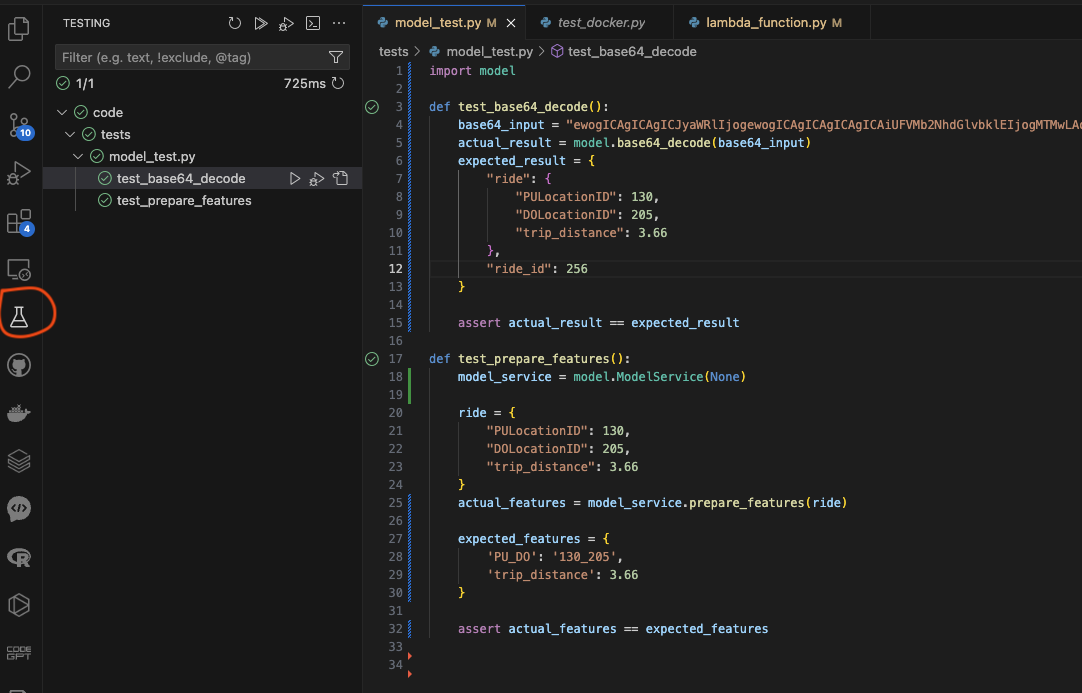
\includegraphics[width=\textwidth]{Images/unit-test-on-vscode.png}
	\caption{Running Pytest on VSCode}
	\label{fig:16}
\end{figure}
\FloatBarrier

To perform unit test on terminal, run \smtt{pipenv run pytest tests/}. This should output the image in \textbf{Fig. \ref{fig:17}} showing that two test ran in the ``tests'' folder and the two test passed.

\begin{figure}[h]
	\centering
	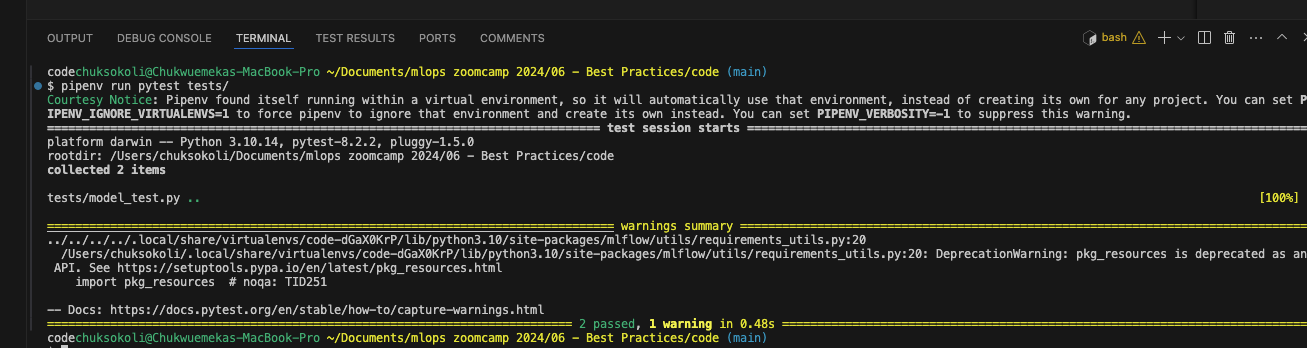
\includegraphics[width=\textwidth]{Images/unit-test-on-terminal.png}
	\caption{Running Pytest on terminal}
	\label{fig:17}
\end{figure}
\FloatBarrier

\section{Integration tests with docker-compose}
To perform integration test with docker-compose, we first build the docker image
\begin{lstlisting}[language=python, numbers=none]
docker build -t stream-model-duration:v2 .

docker run -it --rm \
    -p 8080:8080 \
    -e PREDICTIONS_STREAM_NAME="ride_predictions" \
    -e RUN_ID="e1efc53e9bd149078b0c12aeaa6365df" \
    -e TEST_RUN="True" \
    -e AWS_DEFAULT_REGION="eu-west-1" \
    stream-model-duration:v2
\end{lstlisting}
From a different terminal, we run \smtt{python test\_docker.py}. This runs the fetches the model from S3, runs the model, decode the result and test the output.




\end{document}

